\documentclass[8pt]{extarticle} % or extreport, extbook, depending on your document type
\usepackage{booktabs}
\usepackage[T1]{fontenc} % Recommended for better font encoding
\usepackage[utf8]{inputenc} % Encoding for special characters
\usepackage{blindtext}
\usepackage{multicol}
\usepackage{amsmath}
\usepackage[margin=0.5cm]{geometry}
\usepackage{amssymb}
\usepackage{mathtools}
\usepackage{graphicx}  % For including images
\usepackage{enumitem}
% \usepackage{savetrees}
\linespread{0.8} % 1.5x line spacing
\setlength{\abovedisplayskip}{0pt}
\setlength{\belowdisplayskip}{0pt}

% Reduce space between sections and subsections
\usepackage[compact]{titlesec}
\titlespacing{\section}{0pt}{*0}{*0}  % Zero spacing for sections
\titlespacing{\subsection}{0pt}{*0}{*0}  % Zero spacing for subsections
\titlespacing{\subsubsection}{0pt}{*0}{*0}  % Zero spacing for subsections

% Reduce line spacing
\usepackage{setspace}
\setstretch{0.9}  % Slightly less than single spacing

% Reduce paragraph spacing
\usepackage{parskip}
\setlength{\parskip}{0pt}  % No extra spacing between paragraphs
\setlength{\parindent}{0pt}  % No paragraph indentation

% Compact itemize and enumerate lists
\usepackage{enumitem}
\setlist[itemize]{noitemsep}  % No space between items in itemize lists
\setlist[enumerate]{noitemsep}  % No space between items in enumerate lists



\setlength{\parindent}{0pt}

\begin{document}
\begin{multicols*}{3}

\subsubsection*{Semantic Ambiguity}
Same trees have different meaning
\begin{itemize}[label=\textbullet, labelsep=0.3em, leftmargin=0.5em, itemsep=0em]
    \item \textit{Discourse}: The meeting is cancelled. Nicholas isn't coming into the office today.
    \item \textit{Word senses}: bank (finance or river)
    \item \textit{Quantifier scope}: Every child loves some movie
\end{itemize}

\subsubsection*{Structural (syntactic) Ambiguity}
Different trees produce the same sentence. \\

\underline{POS ambiguities}
\begin{itemize}[label=\textbullet, labelsep=0.3em, leftmargin=0.5em, itemsep=0em]
    \item \textit{Homophones}: blew and blue (particularly in speech)
    \item \textit{Homonyms}: chair (noun or verb)
\end{itemize}
\underline{Attachement ambiguities}:
\begin{itemize}[label=\textbullet, labelsep=0.3em, leftmargin=0.5em, itemsep=0em]
    \item \textit{PP-attachement}: I saw a girl with a telescope\\
$n$ preposition phrases have \\$\operatorname{Cat}_n = \left(\begin{array}{c}2 n \\ n\end{array}\right)-\left(\begin{array}{c}2 n \\ n-1\end{array}\right) \approx \frac{4^n}{n^{3 / 2} \sqrt{\pi}}$ different parses.\\
    \item \textit{Reference}: John dropped the goblet onto the glass table and it broke
\end{itemize}

\begin{center}
    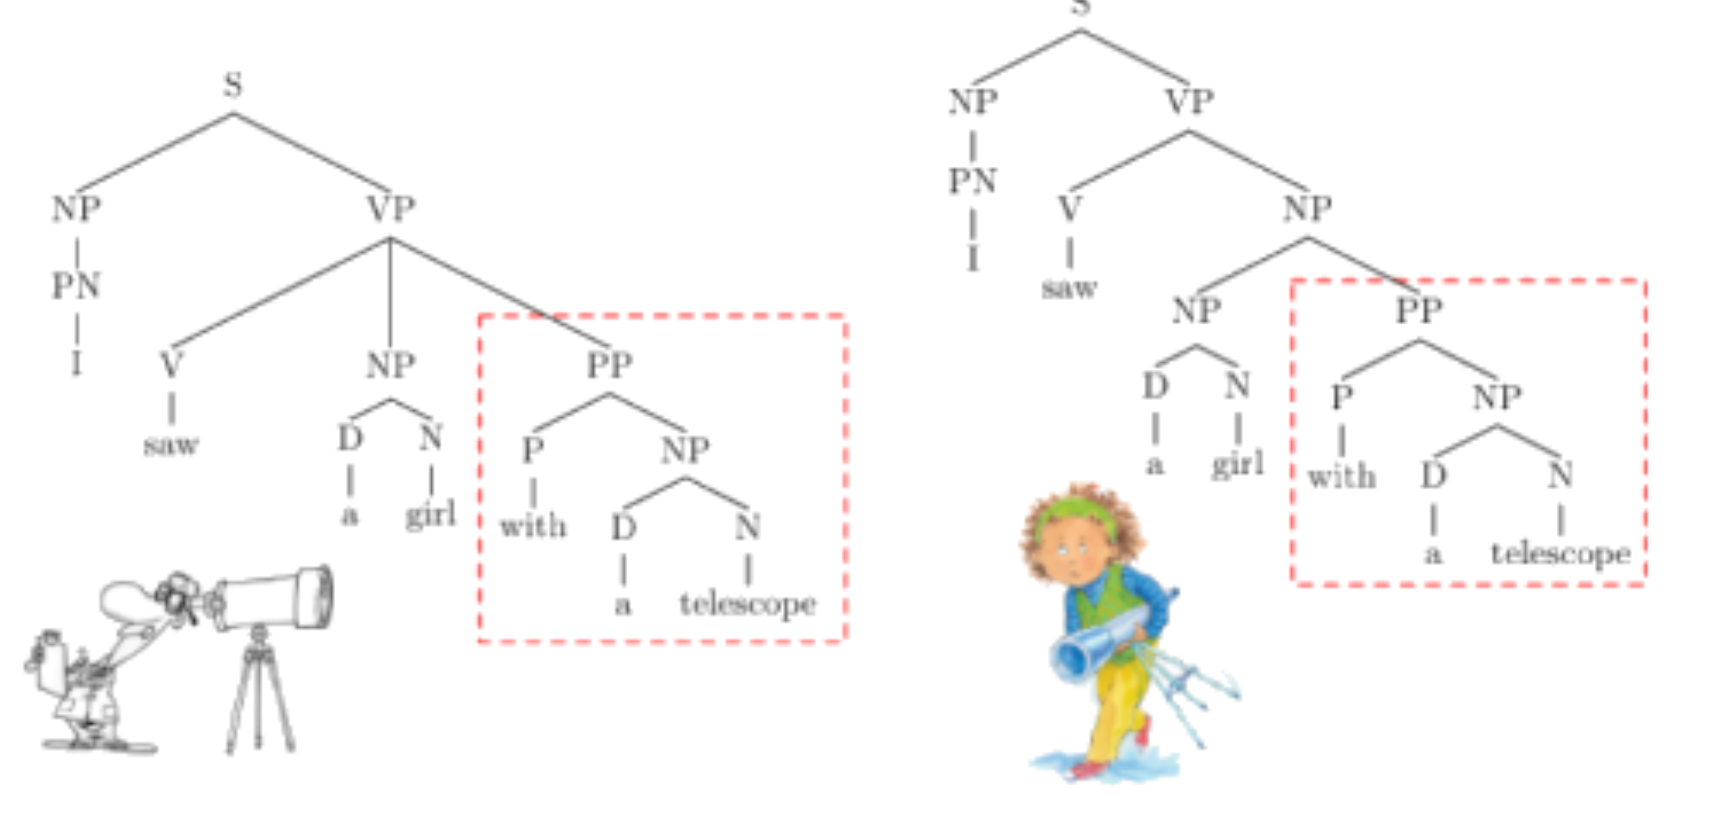
\includegraphics[width=0.3\textwidth]{media/girl.png}
\end{center}

\subsubsection*{Variability}
Multiple different sentences can have the same meaning. 
\begin{itemize}[label=\textbullet, labelsep=0.3em, leftmargin=0.5em, itemsep=0em]
    \item He drew the house
    \item He made a sketch of the house
    \item He portrayed the house in his paintings
\end{itemize}

\subsubsection*{Zipf's Law}
Infrequent words will make up the significant majority of the corpora.
For this reason models have to estimate probabilities for things we rarely or never see in training.
$$f\times r\approx k$$
$$\log f = \log k - \log r$$
- $f$ : frequency of a word\\
- $r$ : rank of a word (if sorted by frequency)\\
- $k$ : constant

\subsubsection*{Checking for Constiuency}
These are groups of words or phrases that can
\begin{itemize}[label=\textbullet, labelsep=0.3em, leftmargin=0.5em, itemsep=0em]
\item be used with conjunction words like and, or, and but. (e.g. washed and peeled)
\item substitute one word or phrase for another (e.g. "it" for NP).
\item appear in the frame "$\_\_\_\_$ is/are/who/what/\\where/when/why/how \ldots'' e.g.
\end{itemize}   
\textit{They put the boxes} in the basement.\\
In the basement is where \textit{they put the boxes}. 

\subsubsection*{Other Reasons}
\begin{itemize}[label=\textbullet, labelsep=0.3em, leftmargin=0.5em, itemsep=0em]
\item Context Dependence
\item Unknown representation
\item Diversity in Language (POS order, number of noun cases (he/him in english, 10+ in russian))
\end{itemize}
Language is not determinsitic hence FSMs and CYK are useful. 

\subsection*{Context/Coprpora}
\begin{itemize}[label=\textbullet, labelsep=0.3em, leftmargin=0.5em, itemsep=0em]
    \item Topic (sports, politics science)
    \item Mode of communication (speech, writing)
    \item Genre (news, fiction, scientific)
    \item Audience (formality, complexity)
\end{itemize}
Important to choose a corpus relevant to the task.

\subsubsection*{Human Annotation / Gold Lables}
Often included in the \textit{metadata} of a corpus.\\
Ofted used as \textbf{gold labels}, the best possible labels for a corpus. Gold labels are not always perfect people make mistakes.
To resolve we must consider
\begin{itemize}[label=\textbullet, labelsep=0.3em, leftmargin=0.5em, itemsep=0em]
    \item Inter-annotator agreement
    \item Annotation guidelines
    \item Annotation tools
\end{itemize}

\textbf{Sentiment Lexicon} is a list of words with their associated sentiment (good / bad). Used as a tool in sentiment analysis, issues include ambiguity, sarcasm, context dependence. 

\subsection*{Parsing}
\subsubsection*{Converting CFG to CNF}
\begin{itemize}[label=\textbullet, labelsep=0.3em, leftmargin=0.5em, itemsep=0em]
\item Get rid of empty (aka epsilon) productions:$C\rightarrow \epsilon$
\item Get rid of unary rules:$C\rightarrow C_1$, 
\item Break up rules w/ n>2 tags to expand into. (Binarisation) \\
For example, $NP \rightarrow DT\quad NNP\quad VBG$ expanded into the two rules $NP \rightarrow DT\quad NNP\mid VBG$ and $NNP\mid VBG\rightarrow NNP \quad VBG$. 
\end{itemize}

\subsubsection*{Treebank PCFGs Disadvantages}
\begin{itemize}[label=\textbullet, labelsep=0.3em, leftmargin=0.5em, itemsep=0em]
\item Do not ecnode lexical preferences
\item Do not encode structural properties beyond single rules.
\item Close attachement is usually more likely (at least in Penn tree bank) (a PP has attached to the closest possible preceding NP) 
\item No lexical dependencies, Replacing one word with another with the same POS will never result in a different parsing decision.
\end{itemize}

\subsubsection*{Fixing PCFGs}
In vertical Markovization we increased context, in horizontal Markovization we want to reduce it.

\underline{Vertical Markovisation}\\
An approach to enrich grammar. 
Helps PCFGs prioritise different structures such as close attachment over other attachments by giving the extra rules different probabilities depending on ancestors. 
Rule applications depend on past ancestors in the tree (not only parents). 
Improves accuracy.
Example is of vertical order 2. 

\underline{Lexicalisation}\\
Makes grammar more specific but grammar blows up + sparse data. Need to do complex smoothing or increasing emphasis on automatically learned subcategories. 

\begin{center}
    \includegraphics*[width=0.3\textwidth]{media/markovisation.png}
\end{center}

\underline{Lexicalised Constituency Parse}\\
Take lexicalised tree and remove phrasal categories i.e S-saw -> saw. Remove duplicated terminals. Continue to collapse chains of duplicates.\\
\textbf{Viterbi} has runtime $O(Tn^2)$ for a sequence of $T$ words and $n$ tags. 

\subsection*{Dependecy Parsing}
\begin{itemize}[label=\textbullet, labelsep=0.3em, leftmargin=0.5em, itemsep=0em]
\item Graph-based: starting from a fully connected graph of all possible edges between constituents, build the minimum spanning tree with the highest total score using edge-factored models. $O(n^2)$
\item Transition-based: use a shift-reduce parser, training a classifier to decide which of the three possible actions to take in order to connect edges between words on the input buffer.\\
\textit{Shift-reduce}: $O(n)$ projective only
\item Conversion-based: starting from a lexicalised constituency parse of the sentence: remove the phrasal categories, remove the duplicated terminals, and collapse chains of duplicates.
\end{itemize}

\textit{Projective}
\begin{center}
    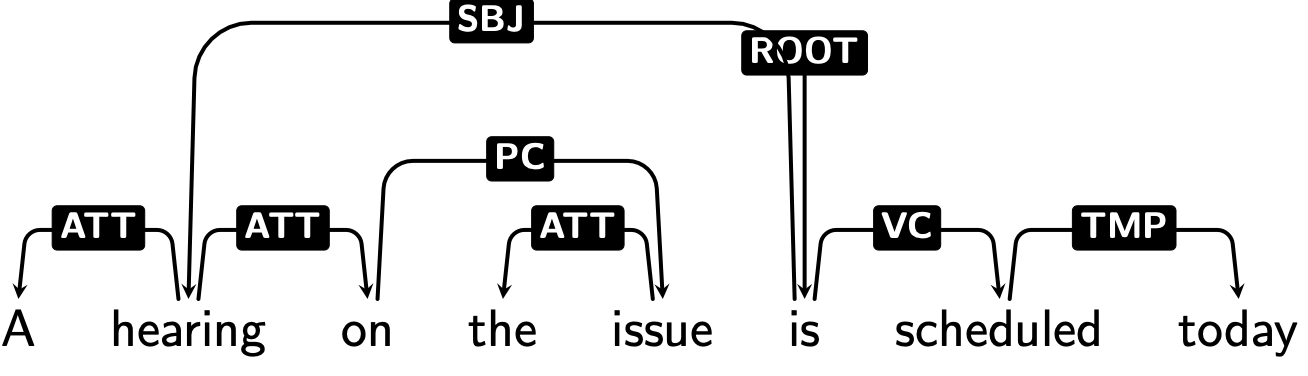
\includegraphics[width=0.3\textwidth]{media/dependency-projective.png}
\end{center}
\textit{Non-projective}
\begin{center}
    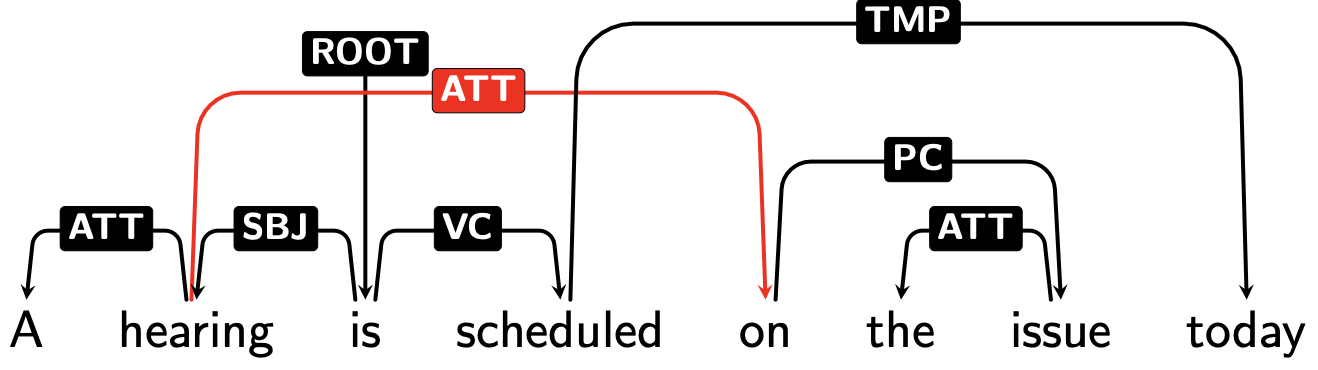
\includegraphics[width=0.3\textwidth]{media/dependency-non-projecitve.png}
\end{center}
Non-projectivity is rare in english.\\
\textit{Examples}
\begin{center}
    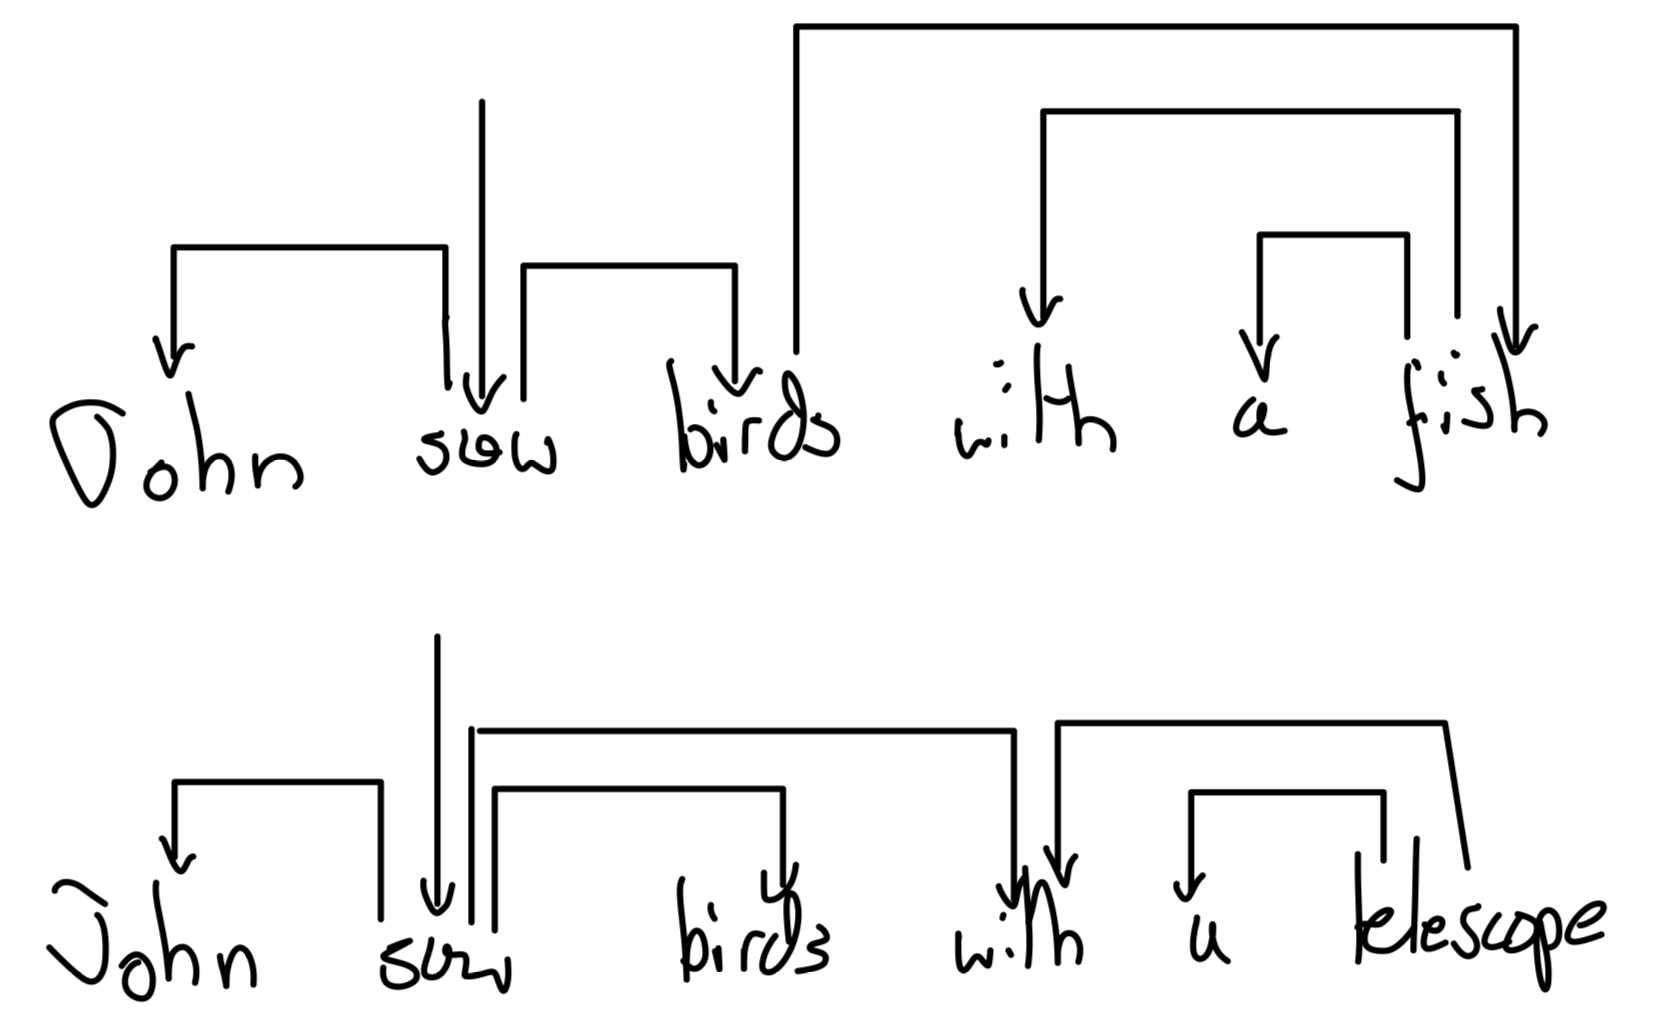
\includegraphics[width=0.3\textwidth]{media/dependency-parse.png}
\end{center}
\underline{Dependency Relations}
\begin{itemize}[label=\textbullet, labelsep=0.3em, leftmargin=0.5em, itemsep=0em]
\item nsubj - nominal/noun subject
\item dobj - direct object
\item amod - adjective modifier
\item advmod - adverbial modifier
\item det - determiner
\item conj - conjunction
\end{itemize}

\subsubsection*{Shift-Reduce}
\begin{center}
    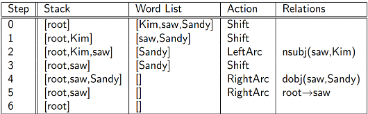
\includegraphics[width=0.3\textwidth]{media/shift-reduce.png}
\end{center}

\underline{Actions}
\begin{itemize}[label=\textbullet, labelsep=0.3em, leftmargin=0.5em, itemsep=0em]
    \item \textit{Shift}: Put w1 on top of the stack.
    \item \textit{LeftArc}: Assign head-dependent relation between s1 and s2; pop s2
    \item \textit{RightArc}: Assign head-dependent relation between s2 and s1; pop s1
\end{itemize}

\subsection*{Compositional Semantics}
\begin{center}
    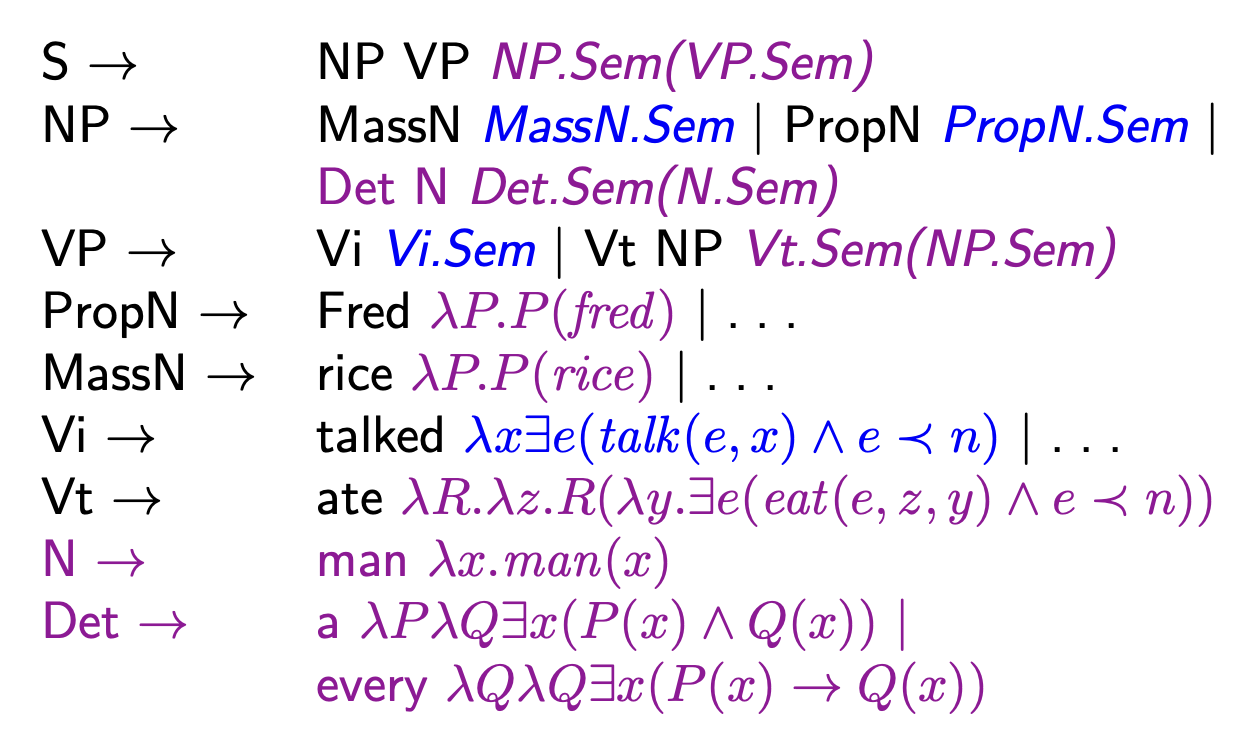
\includegraphics[width=0.3\textwidth]{media/semantic-grammar.png}
\end{center}
\begin{center}
    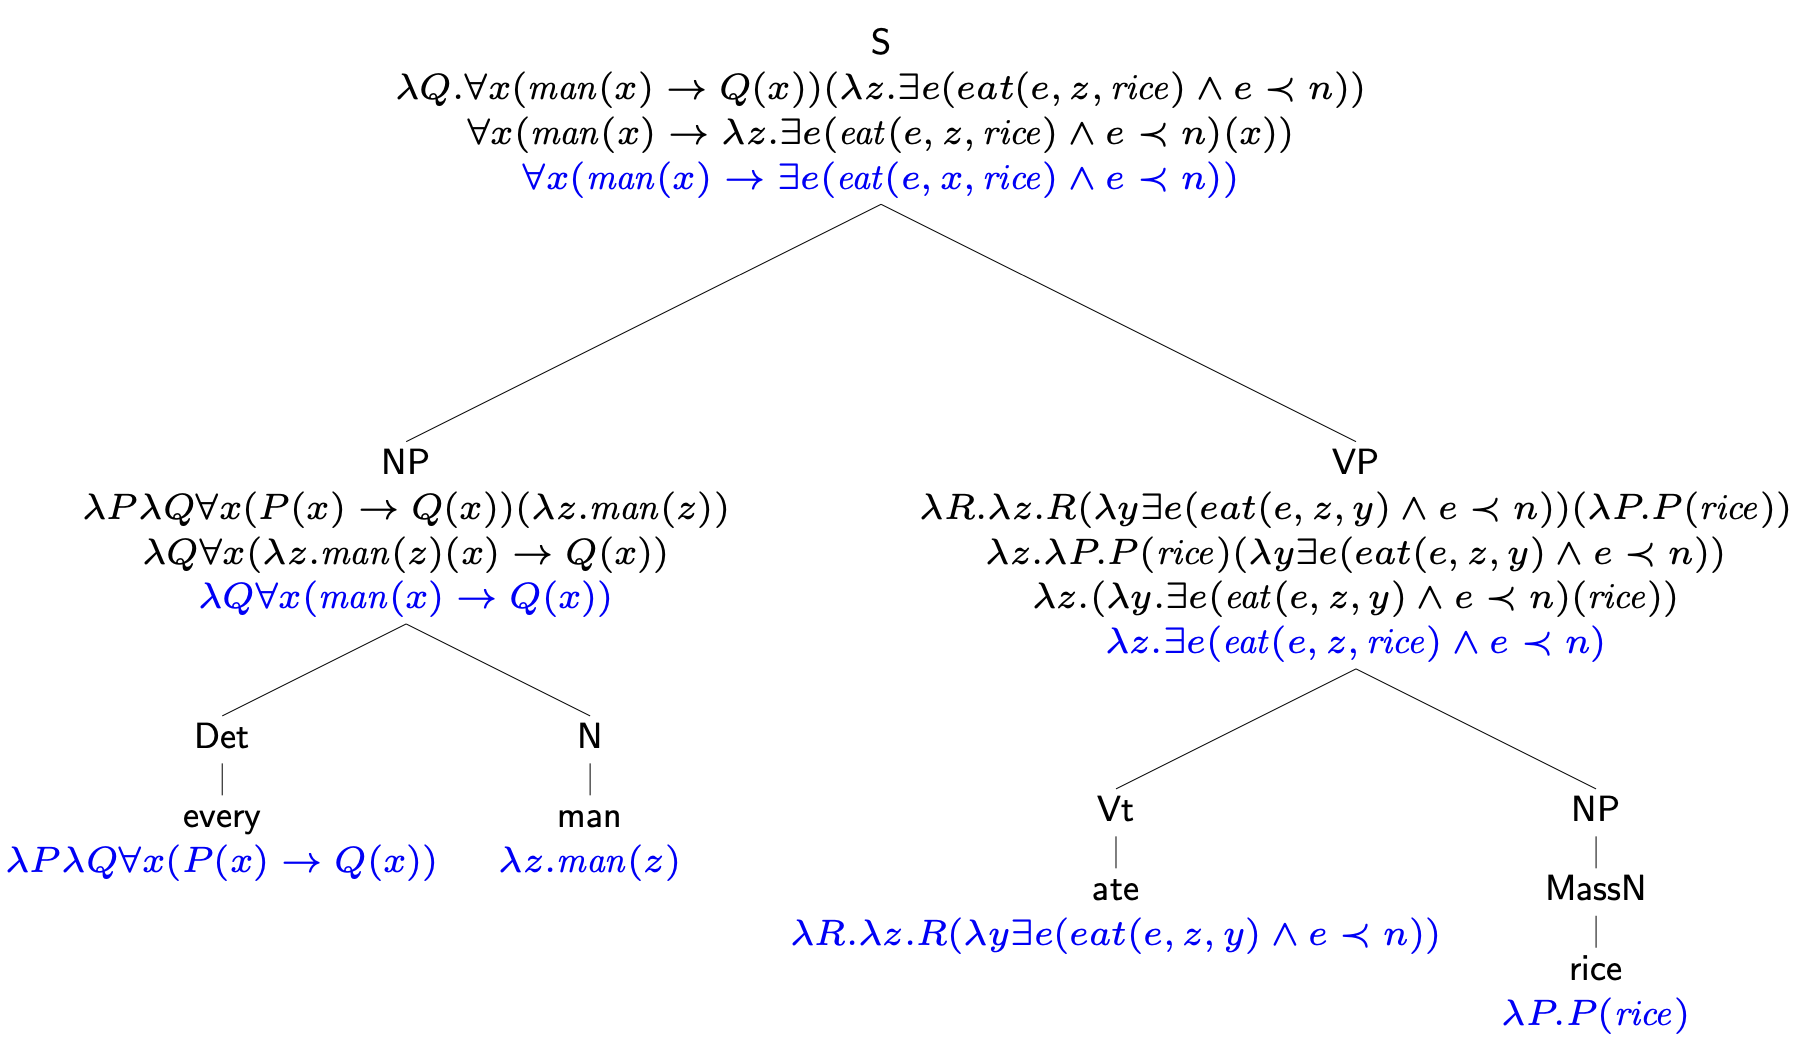
\includegraphics[width=0.3\textwidth]{media/semantic-tree.png}
\end{center}

\subsection*{Linguistics}
In English, whole words are constructed by combining stems and affixes.
\begin{itemize}[label=\textbullet, labelsep=0.3em, leftmargin=0.5em, itemsep=0em]
\item \textbf{Stems}: base (dictionary) words (house, combine, eat, walk, $\ldots$ )
\item \textbf{Affixes}: changes the grammar of a word (prefixes, suffixes, infixes, and circumfixes)
\end{itemize}
Word relations:
\begin{itemize}[label=-, labelsep=0.3em, leftmargin=0.5em, itemsep=0em]
    \item \textbf{Inflection} (stem + grammar affix): no change the grammatical category (walk $\rightarrow$ walking)
    \item \textbf{Derivation} (stem + grammar affix): change to grammatical category (combine $\rightarrow$ combination)
    \item \textbf{Compounding} (stems together): dog, house $\rightarrow$ doghouse
    \item \textbf{Cliticisation}: I've, we're, he's, ...
    \item \textbf{Lemma} of a word is the root $\text{studied}\rightarrow \text{study}$\\
    \item \textbf{Synonyms} words have the same meaning 
    \item \textbf{Meronym} denotes a part of something (leg in chair-leg)
    \item \textbf{Antonym} opposite
    \item \textbf{Hyponym} subset of concept
    \item \textbf{Hypernym} superset of concept 
    \item \textbf{Ontology} a have database of such A is-a B relationships. e.g. WordNet(English)
    \item \textbf{Synset} a set of synonyms. Synsets are connected by hyponym/hypernym/antonym. 
    \item \textbf{Polysemy} Two words with the same form but different meanings with the same origin. e.g. \textit{orange}
    \item \textbf{Homonyms} Two words with the same form but different meanings with different origins. e.g. \textit{bank}
    \item \textbf{Regualr Polysemy} a word a multiple meanings and they are related and this can be predicted because there are other owrds with the saem pattern of meanings. e.g. \textit{orange, cherry}
\end{itemize}
\textbf{Open class words} (content words): nouns, verbs, adverbs, adjectives. Mostly content-bearing: they refer to objects, actions, and features in the world. Open class: new ones are added all the time. \\
\textbf{Closed class words} (function words): pronouns, determiners, prepositions, connectives.\\
Limited num of these. Mostly functional: to tie the concepts of a sentence together.

\subsection*{Word Sense Disambiguation}
This is a classification task. Given a word token in context, which sense (class) does it belong to? 
We can use NB. If features are correlated we use LR. \\

\textbf{Features for WSD}
\begin{itemize}[label=\textbullet, labelsep=0.3em, leftmargin=0.5em, itemsep=0em]
    \item Directly neighboring words (and/or their lemmas)
    \item Content words in a 50 word window
    \item Syntactically related words
    \item Topic of the text
    \item Part-of-speech tag, surrounding part-of-speech tags. 
\end{itemize}

\textbf{Issues with WSD}
\begin{itemize}[label=\textbullet, labelsep=0.3em, leftmargin=0.5em, itemsep=0em]
\item Not always clear how fine-grained the gold-standard should be.
\item Difficult/expensive to annotate corpora with fine-grained senses.
\item Classifiers must be trained separately for each word\\
– Hard to learn anything for infrequent or unseen words\\
– Requires new annotations for each new word\\
– Motivates unsupervised and semi-supervised methods
\end{itemize}

\subsection*{Named Entity Recognition}
Involves recognizing and classifying proper names in text.
\begin{itemize}[label=\textbullet, labelsep=0.3em, leftmargin=0.5em, itemsep=0em]
\item NER systems typically use some form of feature-based sequence tagging, with features like capitalization being important.
\item Lists of known names called gazetteers are also important
\end{itemize}
Different datasets/named entity recognizers use different inventories of classes.\\

\subsubsection*{Types of Classes}
\begin{itemize}[label=\textbullet, labelsep=0.3em, leftmargin=0.5em, itemsep=0em]
\item Smaller: person, organization, location, miscellaneous
\item Larger: sometimes also product, work of art, historical event, etc., as well as numeric value types (time, money, etc.)\\
\end{itemize}

\subsection*{POS Tagging}
Given a string, identify parts of speech.
\begin{itemize}[label=\textbullet, labelsep=0.3em, leftmargin=0.5em, itemsep=0em]
\item A first step towards syntactic analysis and has simpler models that are often faster than full parsing, but sometimes enough to be useful.
\item POS tags can be useful features in text classification or word sense disambiguation. 
\item Hard due to ambiguity and sparse data. The problem of finding the best tag sequence for a sentence is sometimes called decoding because, like spell correction etc, polysemy can also be viewed as a noisy channel model.
\item Corpus annotators decide the num of parts of speech (English 40-100 tags). 
\item Morphologically rich languages often have compound morphosyntactic tags (Noun+A3sg+P2sg+Nom) predicting these requires more complex methods as there are loads of combos. 
\end{itemize}

\subsection*{Spelling Correction}
\textbf{Noisy Channel Model} A message is communicated but noise is introduced and one must decode the noisy message.
\begin{center}
    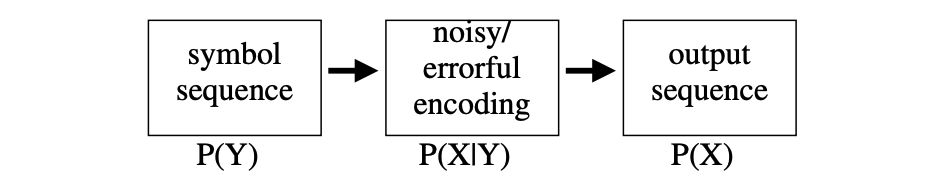
\includegraphics[width=0.3\textwidth]{media/noisy-channel.png}
\end{center}
In spelling correction:
\begin{itemize}[label=\textbullet, labelsep=0.3em, leftmargin=0.5em, itemsep=0em]
\item $P(Y)$ is a distribution over the words which were intended to be typed (a language model).
\item $P(X \mid Y)$ is a distribution describing what the user is likely to type, given what they meant (could use information about common spelling errors). This is the \textbf{noise model}.
\item $P(X)$ is the resulting distribution over what we actually see
\end{itemize}
Formally we want to calculate $\operatorname{argmax}_{y}P(x|y)$.
Using Bayes' Rule we write
$\begin{aligned} 
    \underset{y}{\operatorname{argmax}} P(y \mid x) & =\underset{y}{\operatorname{argmax}} \frac{P(x \mid y) P(y)}{P(x)} \\ 
    & =\underset{y}{\operatorname{argmax}} P(x \mid y) P(y)
\end{aligned}$

\subsubsection*{Basic Spelling Corrction Model}
\begin{itemize}[label=\textbullet, labelsep=0.3em, leftmargin=0.5em, itemsep=0em]
\item Correct each non-word $x_i$ by generating a list of all words $y_i$ that differ by 1 character from $x_i$.
\item Compute $P(\vec{x} \mid \vec{y}) P(\vec{y})$ for each $\vec{y}$ 
\item Returning the $\vec{y}$ with highest value. 
\end{itemize}

\underline{Operations}
\begin{itemize}[label=\textbullet, labelsep=0.3em, leftmargin=0.5em, itemsep=0em]
    \item substitution( $0->e$ )
    \item deletion(t->-)
    \item insertion(-->u)
\end{itemize}
Assuming that the typed character $x_i$ depends only on intended character $y_i$ then
$$
P(\vec{x} \mid \vec{y})=\prod_{i=1}^n P\left(x_i \mid y_i\right)
$$

\underline{Example}\\
$\mathrm{P}($ no $\mid$ not $)=\mathrm{P}(\mathrm{n} \mid \mathrm{n}) \mathrm{P}(\mathrm{o} \mid 0) \mathrm{P}(-\mid \mathrm{t})$
To estimate $P\left(x_i \mid y_i\right)$, count how many times each character (including empty character for del/ins) was used in place of each other character-> confusion matrix. Use MLE or smoothing to estimate probs\\

\subsubsection*{Edit Distance}
All operations have $cost = 1$ apart from substitution between identical letters (unless specified otherwise).
\begin{center}
    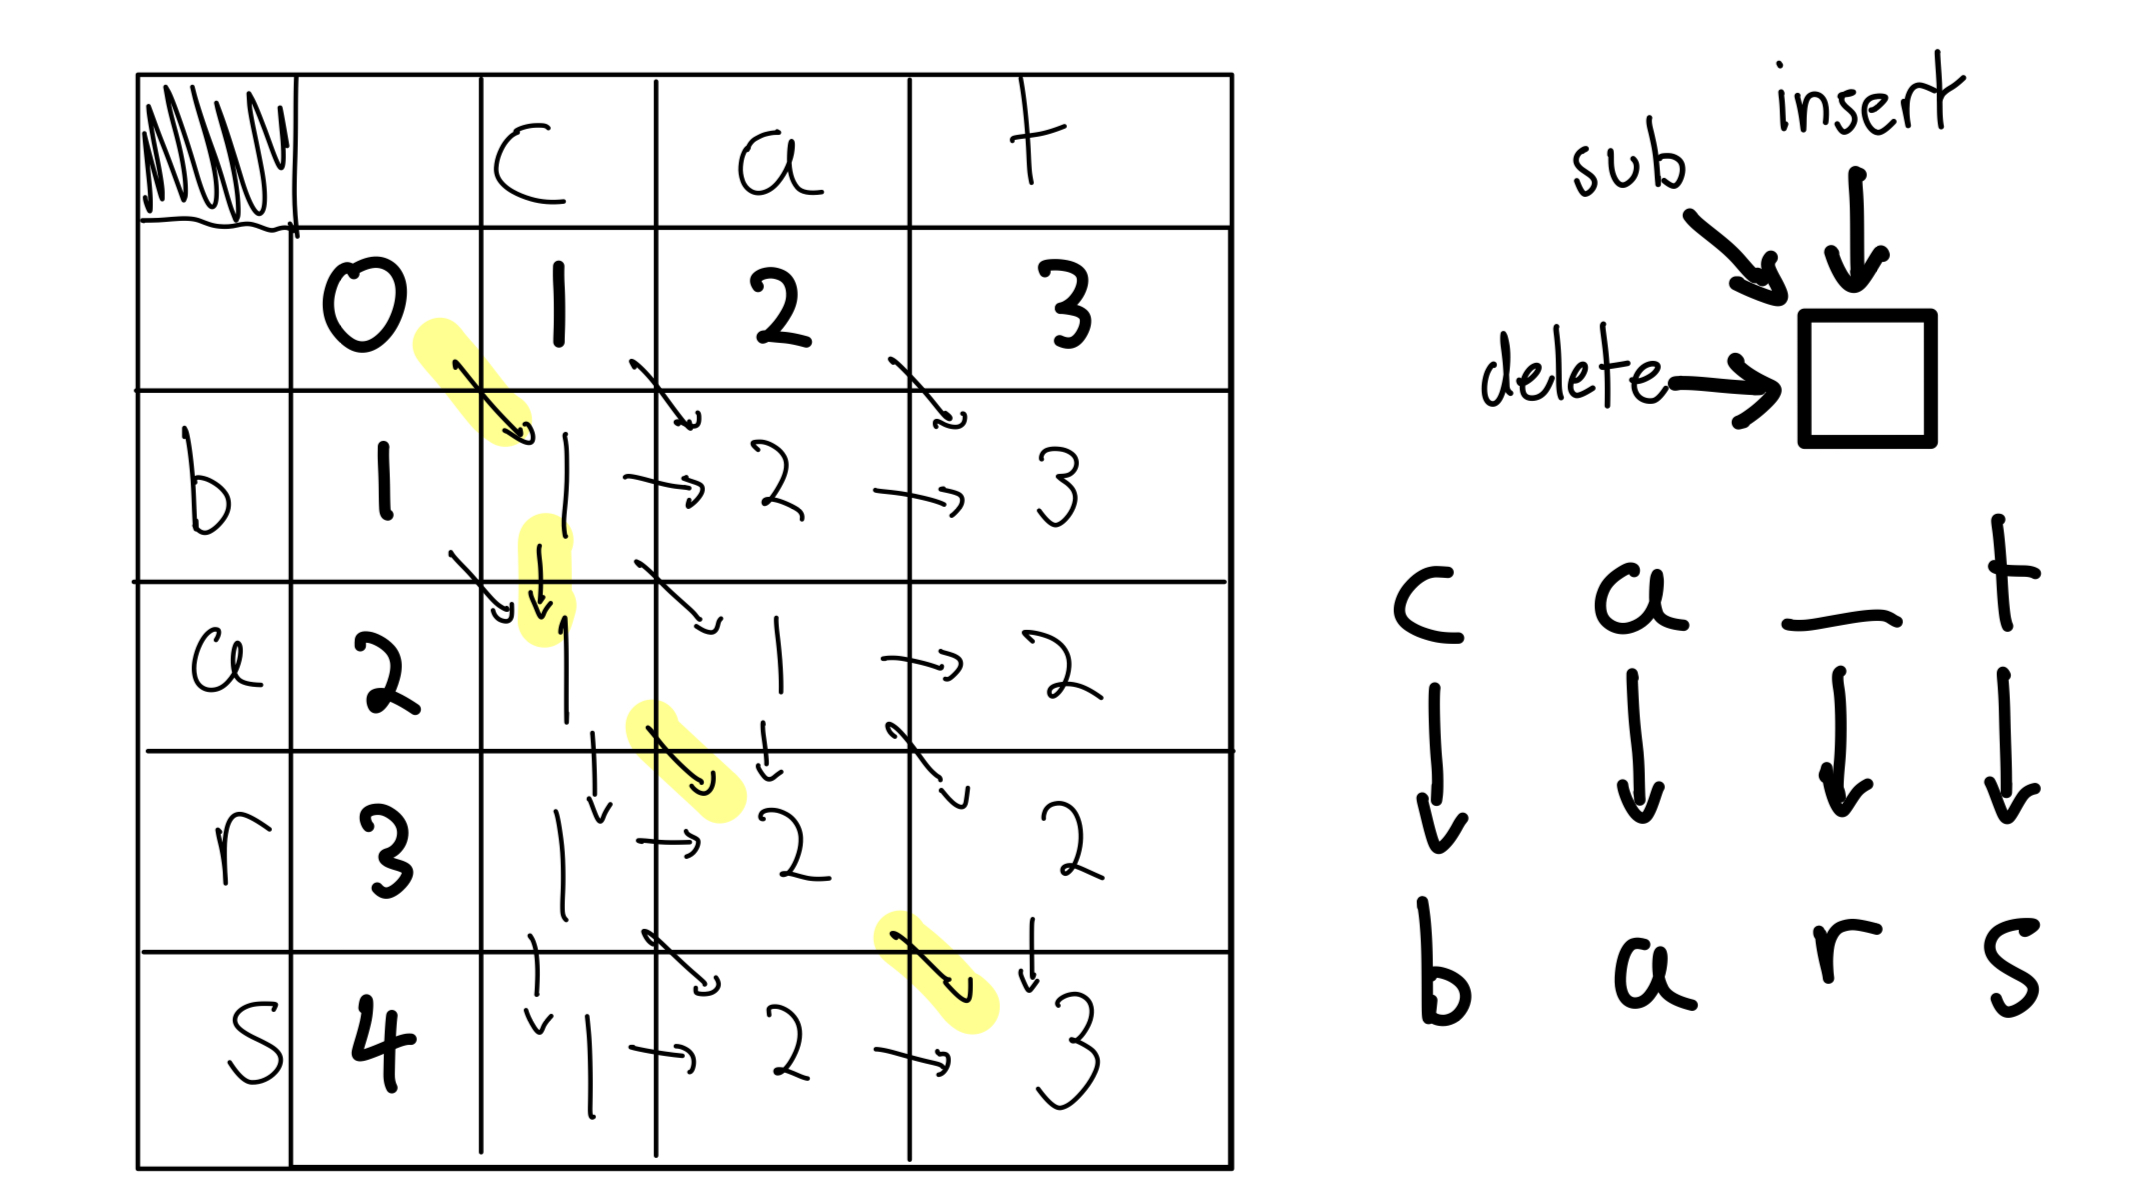
\includegraphics[width=0.3\textwidth]{media/edit.jpg}
\end{center}

\subsection*{N-gram Models}
\begin{itemize}[label=\textbullet, labelsep=0.3em, leftmargin=0.5em, itemsep=0em]
    \item Text-generation
    \item Text-classification
    \item POS-tagging
    \item Named-entity recognition  
\end{itemize}
\textbf{Trigram equation}$$P_{M L E}\left(w_i \mid w_{i-2}, w_{i-1}\right)=\frac{C\left(w_{i-2}, w_{i-1}, w_i\right)}{C\left(w_{i-2}, w_{i-1}\right)}$$
\textit{Start/end of sentence tags} and \textit{costs} are used. 

\textbf{Markov Assumption} the probability of a word only depends of a fixed number $N$ of previous words. 

\textbf{Order} Higher order $N$-grams are more context-sensitive but suffer from sparsity, whereas lower order $N$-grams have reduced context but are less sparse.

\textbf{MLE}$P_{M L E}(x)=\frac{C(x)}{\sum_{x^{\prime}} C\left(x^{\prime}\right)}$

\subsubsection*{Smoothing} 
reduces sparse data problem. Smoothing methods below assign equal prob to all unseen events if interpolation and back-off are not used.\\

\textbf{Add-$\alpha$ (Lidstone) Smoothing}: Add $\alpha$ to all counts and normalise. 
We choose $\alpha<1$ that minimises loss on the dev set. \\
\textit{NB:} $\alpha = 1 \implies$ Laplace smoothing.
\begin{itemize}[label=\textbullet, labelsep=0.3em, leftmargin=0.5em, itemsep=0em]
    \item \textit{Advantages}: simple, easy to implement
    \item \textit{Disadvantages}: overestimates the probability of unseen events, assumes $v$ is known
\end{itemize}
Let $v:=$ vocab size
$$
P_{+\alpha}\left(w_i \mid w_{i-1}\right)=\frac{C\left(w_{i-1}, w_i\right)+\alpha}{C\left(w_{i-1}\right)+\alpha v}
$$
\textbf{Katz-Backoff}: 
If $C(w_{i-1}, w_i)=0$, backoff to lower order $N$-grams, using a \textit{back-off weight} $\alpha$ to choose how the probability mass is distributed. Otherwise just use a discounted probability $P^*$.
\begin{itemize}[label=\textbullet, labelsep=0.3em, leftmargin=0.5em, itemsep=0em]
\item \textit{Advantage}: Looking at smaller n-grams allows us to look at words in less context, allowing the model to generalise to new contexts easier. 
\item \textit{Difference from Good-Turing}: Distribute mass across lower order n-grams using weights instead of uniformly across all unseen n-grams. 
\end{itemize}
\begin{align*}
   &P_{\mathrm{BO}}\left(w_3 \mid w_{1}, w_2 \right)= \\
    &\begin{cases}P^*\left(w_3 \mid w_{1}, w_2 \right), \text { if } C\left(w_{1}, w_2, w_3\right)>0 \\ \alpha_{2} P_{\mathrm{BO}}\left(w_2 \mid w_1\right), \text { otherwise. }\end{cases}
\end{align*}
\textbf{Interpolation}: Combine estimates from all n-grams using weights $\lambda_i$.\\
Each $\lambda_i$ must sum to 1. They can be \textit{constant} or \textit{context-dependent} (i.e. tuned using dev set).
$$\begin{aligned} \hat{P}\left(w_3 \mid w_{1} w_{2}\right)= & \lambda_1 P\left(w_3\right) +\lambda_2 P\left(w_3 \mid w_{2}\right) \\ & +\lambda_3 P\left(w_3 \mid w_{1} w_{2}\right)\end{aligned}$$

\textbf{Good-Turing}: Distribute probability mass unniformly across unseen n-grams. \\
$N_c:=$ number of n-grams seen $c$ times\\
$N:=$ total seen n-grams\\
${c}:=$ actual count\\
$c^*:=$ adjusted count\\
$P^*_c:=$ adjusted probability for an n-gram seen $c$ times.\\
$NB$: If we don't know $N_0$, let $N_0=N_1$ or for bigrams we can \textit{estimate} with $N_0=V^2-N$. 
    $$c^*=(c+1)\frac{N_{c+1}}{N_{c}}\qquad P^{*}_c=\frac{c^{*}}{N}$$

\textbf{Kneser-Ney}: \textbf{no. 1 smoothing method!!}\\
Count how many times a word occured with a unique preceding word (distinct histories) and MLE. \\
Avoids bias in $P(york|new)$.
$$
\begin{gathered}
N_{1+}\left(\bullet w_i\right)=\left|\left\{w_{i-1}: c\left(w_{i-1}, w_i\right)>0\right\}\right| \\
P_{K N}\left(w_i\right)=\frac{N_{1+}\left(\bullet w_i\right)}{\sum_w N_{1+}(\bullet w)}
\end{gathered}
$$

\subsection*{Neural Language Models}
Language modelling with NNs is just a classification problem, given a sequence of previous words, output a probability distribution over next possible words.\\
Vector representation of a text has some dimensionality $d$ but in the end, we need a vector of size $|V|$. The linear layer we apply to the vector representation of the text must then have $|V|$ columns. Each column can be thought of as an \textit{output word embedding}. 
\begin{center}
    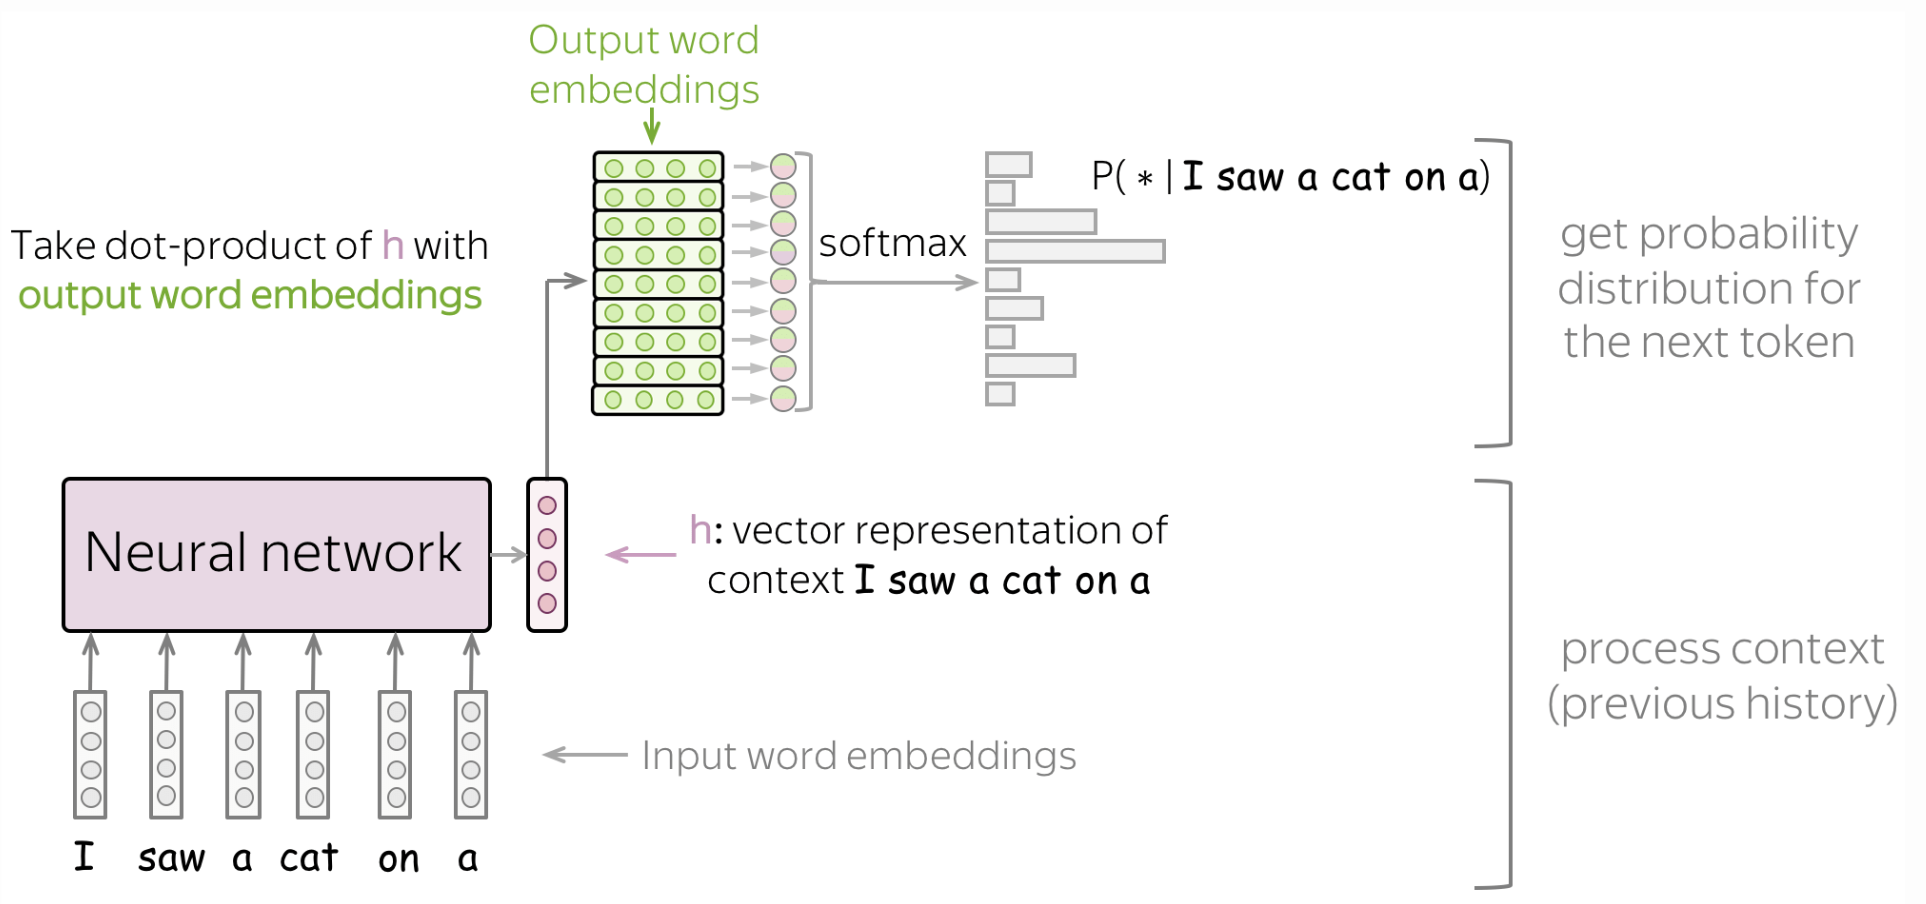
\includegraphics[width=0.3\textwidth]{media/nn-lm.png}
\end{center}

\underline{Training NN LMs}\\
We train using cross entropy loss against the one-hot vector of the correct token, giving the loss function
$$\operatorname{Loss}\left(p^*, p\right)=-\log \left(p_{y_t}\right)=-\log \left(p\left(y_t \mid y_{<t}\right)\right)$$
So for each token in a sequence we increase the weight of the correct\\ 

\underline{Temperature}\\
Choosing the most probable next word in each case leads to boring generations with mostly frequent words. 
We divide the \textbf{SoftMax} by a temperature $\tau$ to make the distribution more uniform.

$$softmax = \frac{\exp \left(\frac{h^T w}{\tau}\right)}{\sum_{w_i \in V} \exp \left(\frac{h^T w_i}{\tau}\right)}$$
\begin{center}
    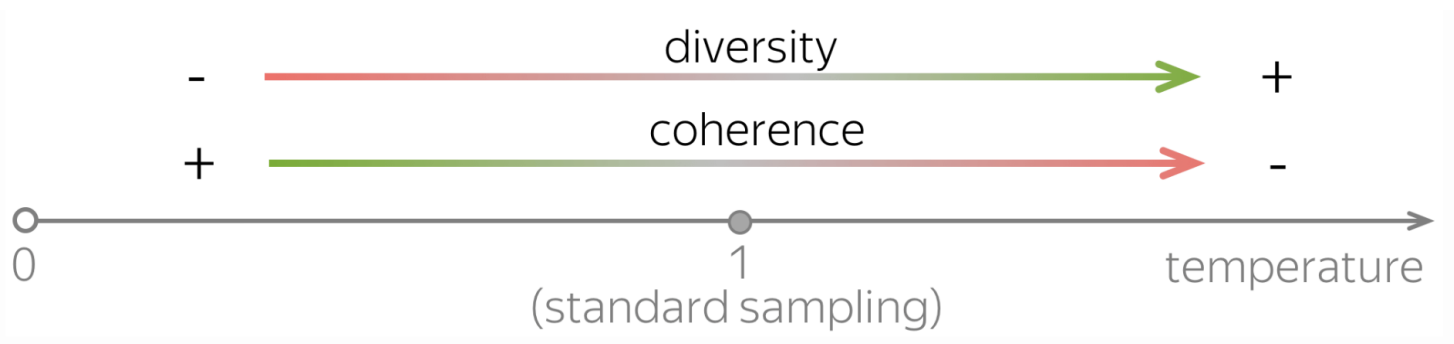
\includegraphics[width=0.3\textwidth]{media/diversity.png}
\end{center}

\subsection*{Evaluation}
\textbf{Extrinsic} measure the performance of a system using a downstream application.

\textbf{Intrinsic} relies on measures inherent to the current task.

\subsubsection*{Metrics for Binary Classification}
${accuracy}=\frac{correct}{total}=\frac{TP+TN}{TP+FP+TN+FN}$\\
$\Uparrow$ doesn't work for imbalanced data i.e. mostly one class.\\
${precision}=\frac{\text{correct +ive tags}}{\text{total tagged}}=\frac{T P}{T P+F P}$\\
${recall}= \frac{\text{correct +ive tags}}{\text{total +ive data}}=\frac{\text{TP}}{\text{TP + FN}}$\\
$F_1=\frac{2 \cdot P \cdot R}{P+R}$

\subsubsection{Metrics for Multi Classification}
\begin{center}
    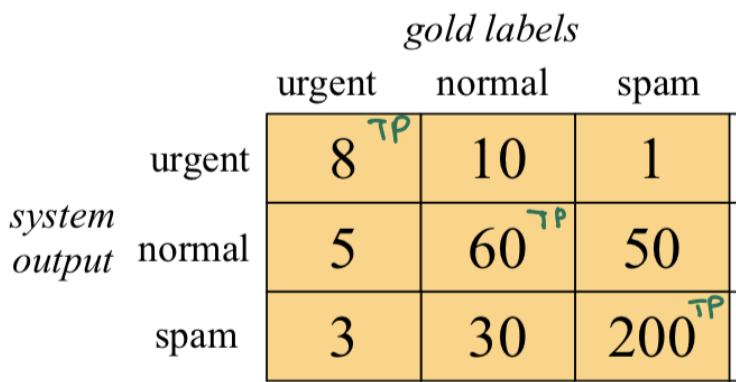
\includegraphics[width=0.3\textwidth]{media/confusion-matrix.png}
\end{center}
Combine precision and recall with micro and macro averaging.
\begin{center}
    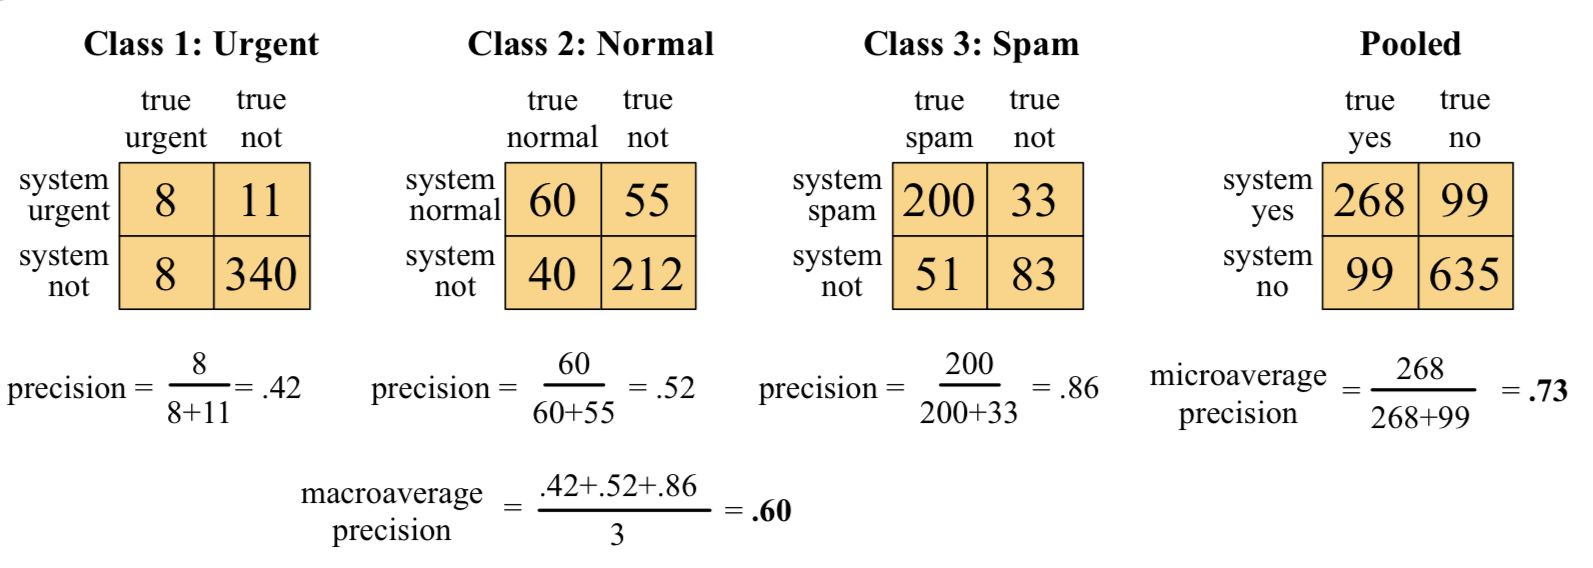
\includegraphics[width=0.3\textwidth]{media/micromacro-averaging.png}
\end{center}

\subsubsection*{Entropy}
Measure of disorder. How many bits (y/n questions we need to find an outcome).
$$H(X)=\sum_x-P(x) \log _2(P(x))$$

\subsubsection*{Cross-Entropy}
Let $P:=$ our model's probability distribution, $\hat{P}:=$ the true distribution.
$$H(P, \hat{P})=\sum_x-P(x) \log _2 \hat{P}(x)$$
$NB$: cross entropy $\geq$ entropy.\\
For a \textit{word sequence} $w_1, \ldots, w_n$, with large $n$, per-word cross-entropy is well approximated by:
$$H_M\left(w_1 \ldots w_n\right)=-\frac{1}{n} \log _2 P_M\left(w_1 \ldots w_n\right)$$

\textbf{Perplexity}:=$2^\text{cross-entropy}$.  LM performance is often reported as perplexity rather than cross-entropy

\subsubsection*{Perplexity vs F-score}
F score allows you to relate the accuracy of the model to the training set (for comparisons with other models and general overview), Entropy/perplexity gives you insight into how the model operates (like the outline of how it reasons and makes decisions)\\

\subsubsection*{Bracket Score}
\begin{center}
    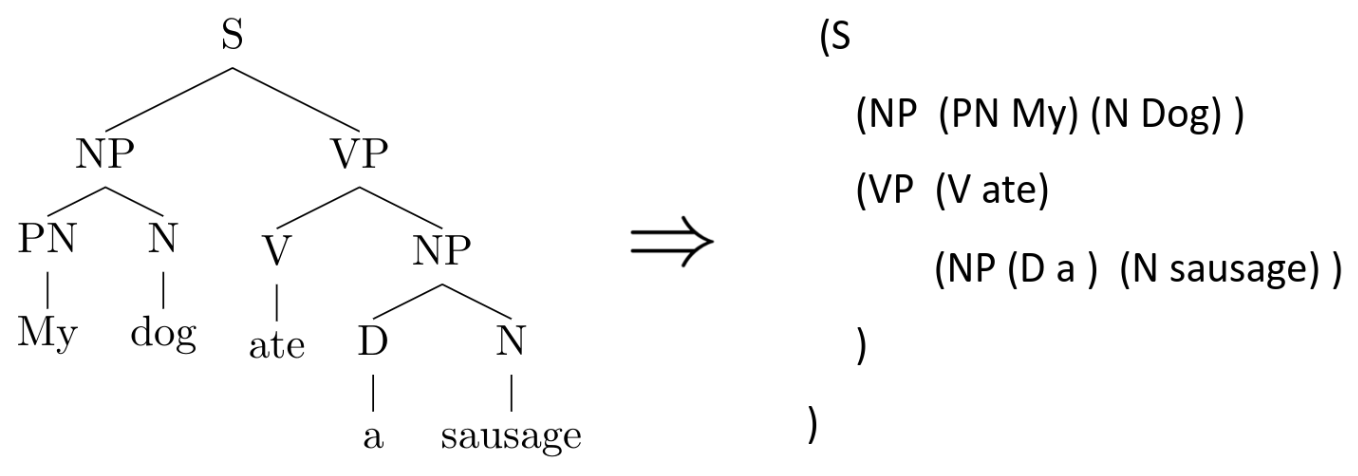
\includegraphics[width=0.3\textwidth]{media/bracket-score.png}
\end{center}
Used to evaluate statistical parsers against gold standard trees, use $F_1$.

\subsubsection*{Expectation Maximisation} 
initialise parameters to an arbitrary value then train a model,
iteratively improve the parameters using newly trained model to 
inform the parameter choice, repeate until there is no change. \\
\underline{Likelihood Function} is $P(data|\theta)$ for parameter $\theta$ of a probabilistic model.\\
\textit{Hard EM} usually converges to the global min, always to the local min. \\
\textit{True EM} always converges to the gloabl min. \\

\subsection*{Classisfication Models}
\subsubsection*{General Structure}
\underline{Feature Extractor}\\
A feature extractor can be either manually defined (as in classical approaches) or learned (e.g., with neural networks).\\

\underline{Classifier}\\
A classifier assigns class probabilities given feature representation of a text. 

\subsubsection*{Naive Bayes}
A generative model. Used for \underline{binary} text-classification. \\
We make a \underline{naive assumption} that features are independent. \\
Features are often just the words in a text. \\

\underline{Classifier}\\
Given a document with features $f_1, f_2, \ldots f_n$ and set of categories $C$, choose the class $\hat{c}$ where
$$
\hat{c}=\underset{c \in C}{\operatorname{argmax}} P(c) \prod_{i=1}^n P\left(f_i \mid c\right)
$$
$P(c)$ := prior probability of class $c$ before observing any data 
(estimated with \textbf{MLE})\\
$P\left(f_i \mid c\right)$ := probability of seeing feature $f_i$ in class $c$ (estimated with MLE and lidstone smoothing).

Or with costs: \\
$\hat{c}=\underset{c \in C}{\operatorname{argmin}}\left(-\log P(c)+\sum_{i=1}^n-\log P\left(f_i \mid c\right)\right)$\\

\underline{NB Derivation}\\
Given document $d$ and set of categories $C$, we want to assign $d$ to the most probable category $\hat{c}$.
$$
\hat{c}=\underset{c \in C}{\operatorname{argmax}} P(c \mid d)
$$
which can be derived to 
$$\begin{aligned} 
    & =\underset{c \in C}{\operatorname{argmax}} \frac{P(d \mid c) P(c)}{P(d)} \\ 
    & =\underset{c \in C}{\operatorname{argmax}} P(d \mid c) P(c)\qquad (*)
\end{aligned}
$$ 
by Bayes' Rule and $d$'s independence from $c$. 
Representing $d$ as the set of features it contains: $f_1, f_2, \ldots f_n$. We have
$$
P(d \mid c)=P\left(f_1, f_2, \ldots f_n \mid c\right)
$$
We then make the naive Bayes assumption that features are conditionally independent given the class
$$P\left(f_1, f_2, \ldots f_n \mid c\right) \approx P\left(f_1 \mid c\right) P\left(f_2 \mid c\right) \ldots P\left(f_n \mid c\right)$$
Substitute this into $(*)$ to get the final equation.

\subsubsection*{Logistic Regression} 
A discriminative model. \\

\underline{Feature Representation in LR}\\
Our text is represented using manually chosen features $f=(f_1\dots,f_n)$ that we think will be helpful for identifying class distinctions.\\
Each is a funtion of our obserbved data $\vec{x}$ (the contents of the text) and a class $c$.\\
Each feature has a \underline{weight} $w_i$.\\

\textit{Example features}:
\begin{itemize}[label=\textbullet, labelsep=0.3em, leftmargin=0.5em, itemsep=0em]
    \item $f_1(\vec{x}, c)=1$ if 'ski' in $\vec{x}$ and $c=1$
    \item $f_4(\vec{x}, c)=1$ if 'expedia.com' is linked to and $c=1$
    \item $f_9(\vec{x}, c)=$ number of links in $\vec{x}$ and $c=3$
\end{itemize}

\underline{LR Classifier (SoftMax)}\\
Unlike Naive Bayes, we model $P(c \mid d)$ directly.\\
We choose the class with the highest probability according to \textbf{SoftMax}
$$
P(c \mid \vec{x})=\frac{\exp \left(\sum_i w_i f_i(\vec{x}, c)\right)}{\sum_{c^{\prime}} \exp \left(\sum_i w_i f_i\left(\vec{x}, c^{\prime}\right)\right)} 
$$
This is equivalent to finding the class for which $\vec{w} \cdot \vec{f}$ is highest.\\

\underline{Training}\\
We need to determine which weights make the labels on our annotated data most probable.\\
We use \textbf{Gradient Descent} to find the weights that minimise the \textbf{Cross-Entropy Loss} of our model.\\

\underline{Cross-Entropy Loss for LR}\\
The true distribution is a one-hot vector $P$, where $P_i=1$ if the class is $i$ and $0$ otherwise.\\
The model distribution $\hat{P}$ is the output of SoftMax.

Since the true distribution is one-hot, for a true class $k$ the cross-entropy loss simplifies to
$$\operatorname{Loss}\left(P, \hat{P}\right)=-\log \left(\hat{P}_k\right)$$

\underline{Gradient Descent}\\
Randomly initialise the weight vector $\vec{w}$ and nudge it in the right direction using derivative of the loss function.
$$
\vec{w} \leftarrow \vec{w}+\eta \cdot \nabla_w \sum_{j=1}^N \log \left(P\left(c^{(j)} \mid x^{(j)}\right)\right)
$$
$\eta$ := learning rate, a hyper parameter of the model. \\

\underline{Mini-batch gradient descent}\\
Like gradient descent but does not sum over all $\mathrm{N}$ on each iteration, only a batch $\mathrm{B}\subset\mathrm{N}$.\\

\textbf{LR vs NB}
\begin{itemize}[label=\textbullet, labelsep=0.3em, leftmargin=0.5em, itemsep=0em]
    \item Both are simple; Naive Bayes is simpler.
    \item Both methods are interpretable: you can look at the features which influenced the predictions most.
    \item Naive Bayes is very fast to train. Logistic regression is slower, you have to go over the data many times until the gradient ascent converges.
    \item Naive Bayes is too "naive", can lead to over confidence. 
    \item Both methods use manually defined feature representation. You are likely to miss something which can be useful for the task.
    \item Logistic Regression is less robust than NB when the test data varies from the training data as it will depend on the presence of other predictive features.
\end{itemize}

\subsubsection*{NNs for Classification}
All neural network classifiers classify the same as LR, using \textbf{softmax}, we just have to use some $linear-layer$ to reduce the dimensionality of our text-representation vector to a vector representing our class distribution. \\
The only difference from LR an clasical models is where the features come from. \\
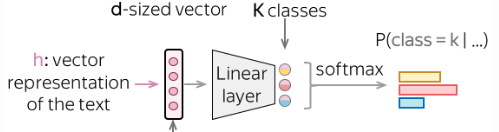
\includegraphics[width=0.35\textwidth]{media/nn-classifier.png}
Generally, we pass the \textbf{Word Embeddings} of the tokens in a document to a NN so it can learn which features represented in the embeddings are relevant for classification. 

\subsubsection*{(Weighted) Bag of Embeddings}
Represnt the text as a sum or weighted sum of the embeddings of the words in the text.\\
Weighted sum could be calculated using $tf-idf$ (see LSA).\\
This (along with NB) should act as a \textbf{baseline} for any NN, if our model cannot do better than this, it's not worth using NNs.

\subsubsection*{RNNs}
Reads a sequence of tokens.\\
At each step we take an input vector (token embedding) and a previous state (which encodes all previous information) and compute a new state. 
\begin{center}
\includegraphics*[width=0.15\textwidth]{media/rnn-cell.png}
\end{center}
The RNN cell (the stuff doing the encoding) is the same at all steps.\\
The output vector must be the last state - only this state saw all input tokens.\\  

\underline{Vanilla RNN}\\
Transforms $h_{t-1}$ and $x_t$ linearly then applies a non-linearity (e.g. $\tanh$) 
\begin{center}
\includegraphics*[width=0.25\textwidth]{media/vanilla-rnn.png}
\end{center}
\textit{Disadvantage}: suffer from vanishing and exploding gradients problem.\\

\underline{Multi-layer RNNs}\\
Stack multiple layers, inputs for the higher RNN are representations from the previous layer.\\

The main hypothesis is that lower layers catch local phenomena (e.g., phrases), higher layers learn high-level things (e.g. topic).
\begin{center}
\includegraphics*[width=0.25\textwidth]{media/multi-layer.png}
\end{center}
\textit{Disadvantage}: the last state can easily "forget" earlier tokens.\\

\underline{Bi-directional}\\
To help with "remembering" earlier vectors we can use a \textit{forward} RNN that reads left to right and a \textit{backward} RNN that reads right to left.\\

We combine the output vectors of both (sum, contatenate, etc.) 
\begin{center}
\includegraphics*[width=0.25\textwidth]{media/bi-directional.png}
\end{center}

\textit{Disadvantage:} when stacking a lot of layers, you can have a problem with
propagating gradients from top to bottom through a deep network. 
To mitigate, this we use \textit{Residual} or \textit{Highway} connections which add a block's input to its output.

\subsubsection*{Conv Nets}
Conv nets are used when we are looking for patterns in a text but don't care where they are (e.g. sentiment classification).\\

\underline{Step 1: Convolution}\\
\begin{center}
\includegraphics*[width=0.24\textwidth]{media/conv-net1.png}
\end{center}
$k$ := kernel size;\\
$m$ := output channels\\
$d$ := inpute channels (i.e. embedding dimension)\\

We apply a linear layer $W\in\mathbb{R^(k\cdot d)\times m}$ to a concatenation of $k$ input vectors $u_i=\left[x_i, \ldots x_{i+k-1}\right]$. So for one convolution we have
$$F_i = u_i \times W$$
Each column in $W$ corresponds to a feature or output channel.\\

\underline{Step 2: Pooling}\\
Polling layer summarises each of the $m$ features in some region.

\textit{Max-pooling} takes the maximum of each feature.

\textit{Mean-pooling} computes mean over each feature.

\textit{Pool size} controls how many convolutions we pool over, \textit{stride} size controls how "far apart" each pool is.

For text classification we usually use \textit{global-over-time pooling} which compresses the text into a single vector. \\

\underline{Practical Tricks}\\
\textit{Concatenate reuslts of multiple kernal sizes}
\begin{center}
\includegraphics*[width=0.25\textwidth]{media/multiple-kers.png}
\end{center}
\textit{Multiple Layers}
\begin{center}
\includegraphics*[width=0.25\textwidth]{media/multiple-layers.png}
\end{center}
Useful for
\begin{itemize}[label=\textbullet, labelsep=0.3em, leftmargin=0.5em, itemsep=0em]
    \item Long documents
    \item Models which start with character embeddings rather than words
    \item In principle, complex tasks, requiring modeling interaction
    between patterns
\end{itemize}

\subsection*{Word Embeddings}
A word embedding is a vector representation of a word, typically one where proximity in vector space correlates to a similarity in meaning.
\subsubsection*{Analogous Embeddings}
For an analogy $a:b:: a^*: b^*$ ($a$ is to $b$ as $a^*$ is to $b^*$) we have 
$$
\overrightarrow{\mathrm{b}} *=\operatorname{argmin} \text { distance } \overrightarrow{\mathrm{x}}(\overrightarrow{\mathrm{x}}, \overrightarrow{\mathrm{b}}-\overrightarrow{\mathrm{a}}+\overrightarrow{\mathrm{a}} *)
$$
\subsubsection*{Distance Metrics}
\begin{itemize}[label=\textbullet, labelsep=0.3em, leftmargin=0.5em, itemsep=0em]
    \item \textit{Euclidean}: $E D(\vec{u}, \vec{v})=\sqrt{\sum_{i=1}^d\left(\vec{v}_i-\vec{u}_i\right)^2}$
    \item \textit{Cosine Similarity}: $\cos \left(\theta_{\vec{w} \vec{v}}\right)=\frac{\vec{v} \cdot \vec{w}}{|\vec{v}||\vec{w}|}$\\
The cosine similarity represents the cosine of the angle between two input vectors, and is equivalent to the normalised dot product. \\
Cosine Distance = 1 - Cosine Similarity
    \item \textit{Dot Product}: $\operatorname{dot}(\vec{u}, \vec{v})=\sum_{i=1}^d \vec{u}_i \vec{v}_i$
\end{itemize}
\textit{comparing Cosine and Euclidian Distance}:\\
Two vectors in the same direction can be very distant as per the Euclidean distance, but still very similar according to the cosine similarity. \\
However, for normalised vectors, they are related, as is illustrated below\\
If $\vec{u}$ and $\vec{v}$ have length $1, E D(\vec{u}, \vec{v})^2=$ $2-2 \operatorname{dot}(\vec{u}, \vec{v})$.
$$
\begin{aligned}
E D(\vec{u}, \vec{v}) & =\sqrt{\sum_{i=1}^d\left(\vec{v}_i-\vec{u}_i\right)^2} \\
&=\sqrt{\sum_{i=1}^d \vec{v}_i \vec{v}_i+\sum_{i=1}^d \vec{u}_i \vec{u}_i-2 \sum_{i=1}^d \vec{v}_i \vec{u}_i} \\
E D(\vec{u}, \vec{v})^2 & =\sum_{i=1}^d \vec{v}_i \vec{v}_i+\sum_{i=1}^d \vec{u}_i \vec{u}_i-2 \sum_{i=1}^d \vec{v}_i \vec{u}_i\\
&=\|\vec{v}\|^2+\|\vec{u}\|^2-2 \operatorname{dot}(\vec{u}, \vec{v})\\
&=2-2\operatorname{dot}(\vec{u}, \vec{v})
\end{aligned}
$$

\textbf{One-hot Word Vectors} store each word by having the embedding dimension be equal to the vocabulary size, and having each vector be many zeros and a single one in a position corresponding to that word.

\subsubsection*{Count-based Methods}
We have to put information about contexts into word vectors manually based on global corpus statistics.\\

Two steps: 
\begin{itemize}[label=\textbullet, labelsep=0.3em, leftmargin=0.5em, itemsep=0em]
    \item construct a word-context matrix with a \underline{context} and a way of quantifying association between words and contexts, i.e. a formula for computing \underline{matrix elements}
    \item reduce its dimensionality with SVD
\end{itemize}

\textbf{SVD} (Singular Value Decomposition) is a method for finding the most important dimensions of a data set.\\
\textit{Advanatges}\\
- smaller matrix allows for cheaper computation\\
- a lot of words appear in only a few of possible contexts, SVD removes a lot of uninformative elements (e.g., zeros).\\

\subsubsection*{Co-occurence Counts} 
\underline{Context}: surrounding words in a L-sized window\\
\underline{Matrix element}: $N(w, c)$ - number of times word w appears in context c\\

\subsubsection*{Positive Pointwise Mutual Information (PPMI)}
\underline{Context}: surrounding words in a L-sized window\\
\underline{Matrix element}: $PPMI(w, c)=\max (0, \mathrm{PMI}(\mathrm{w}, \mathrm{c}))$\\ where \\
$\mathrm{PMI}(\mathrm{w}, \mathrm{c})=\log \frac{P(\mathrm{w}, \mathrm{c})}{P(\mathrm{w}) P(\mathrm{c})}=\log \frac{\mathrm{N}(\mathrm{w}, \mathrm{c})|(\mathrm{w}, \mathrm{c})|}{\mathrm{N}(\mathrm{w}) \mathrm{N}(\mathrm{c})}$\\

\subsubsection*{LSA} (Latent Semantic Analysis)
\underline{Context}: a full document $d$ from a collection of documents $D$\\
\underline{Matrix element}: $tf-idf(w, d, D) = tf(w, d) \cdot idf(w, D)$
$tf-idf$ is defiend\\
- $tf(w, d)$: count of word $w$ in document $d$\\
- $idf(w, D)$ := $\log \frac{|D|}{|\{d \in D: w \in d\}|}$(inverse document frequency)\\

LSA is hard to scale even when we reduce its dimensionality.

\subsubsection*{Prediction-based Methods}
\textbf{Word2Vec} is a collection of different models which convert words into their word embeddings. 

\subsubsection*{Skip-gram} 
\begin{center}
    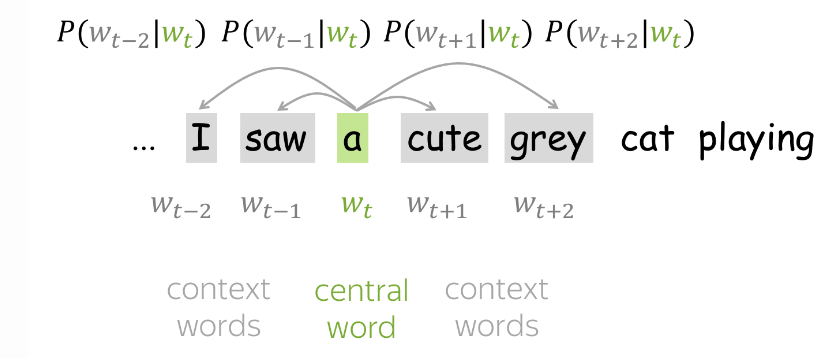
\includegraphics[width=0.3\textwidth]{media/skipgram.png}
\end{center}
\begin{itemize}
    \item go over the text with a sliding window, moving one word at a time.\\
    At each step, there is a \underline{central word} and \underline{context words} (other words in this window);
    \item for the central word, compute probabilities of context words;
    \item adjust the vectors to increase these probabilities (gradient descent).
\end{itemize}

\underline{Loss Function}\\
We use the \textit{average negative log liklelihood} of all of our preditions at each time step $t= 1\dots T$
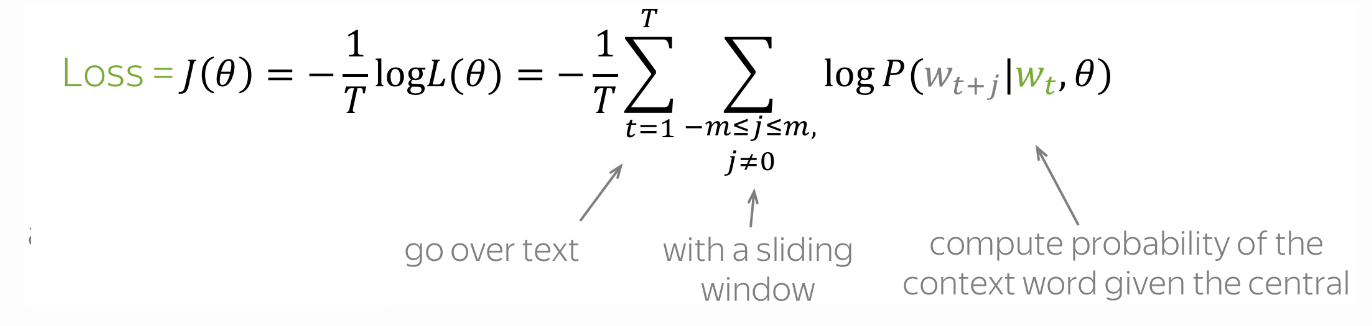
\includegraphics[width=0.35\textwidth]{media/skigram-loss.png}

\underline{Calculating $P(w_{t+j}\mid w_t;\theta)$}\\
For each word $w$ we have two emedding vectors:\\
- $v_w$ when it is a central word\\
- $u_w$ when it is a context word\\
Once the vectors are trained, usually we throw away context vectors and use only word vectors.\\
The collection of all of these embedidng vectors make up the model's parameters $\theta$.\\

We then calculate $P(w_{t+j}\mid w_t;\theta)$ using \textbf{SoftMax} over the dot product similarity of the context and central vectors
$$P(w_{t+j}\mid w_t;\theta)=\frac{\exp(u_{w_{t+j}}^T v_{w_t})}{\sum_{w \in V}\exp(u_w^T v_{w_t})}$$
Hence for a particular central and context word, i.e. letting $J_{t,j} = -\log P(w{t+j}\mid w_t;\theta)$ :
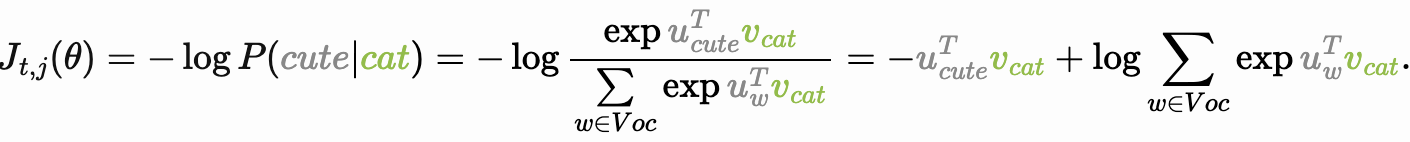
\includegraphics[width=0.33\textwidth]{media/loss-word-context.png}

\underline{Negative Sampling}\\
We can train faster (smaller "steps" in gradient descent but quicker calculation) by decreasing similarity between central 
and context vectors not for all words, but only with a subset of $K$ \textbf{negative samples}.\\

Samples are chosen from the unigram distribution of the corpus, often modified to choose less frequent words more often. \\

\underline{Negative Sampling Loss Function}\\
For a particular central and context word, i.e. letting $J_{t,j} = -\log P(w{t+j}\mid w_t;\theta)$, we have
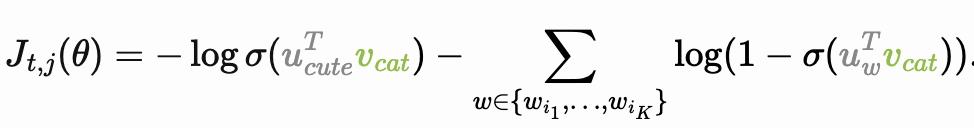
\includegraphics[width=0.33\textwidth]{media/negative-sampling-loss.png}

\textbf{Continuous Bag of Words (CBOW)} is another Word2Vec varient and predicts the central word from the sum of context vectors. This simple sum of word vectors is called "bag of words", which gives the name for the model.

\subsubsection*{Effect of Window Size}
Larger windows tend to produce more topical similarities \\
- e.g. dog, bark, leash or walked, run, walking\\
Smaller windows tend to produce more functional and syntactic similarities \\
- e.g. Poodle, Pitbull, Rottweiler, or walking, running, approaching\\


\subsection*{Sequence to Sequence}
\subsubsection*{Encoder Decoder Framework}
\underline{encoder} processes the input text in the source language, 
understanding its grammar, vocabulary, and nuances. \\
\underline{decoder} generates the translated text in the target language, given the translated text up 
to that point and the vector representation of the input text. \\

Having separate modules allows each to specialise and optimise for their respective languages. Also, separating the encoder and decoder adds flexibility to the machine translation system. \\

\underline{Simple RNN Based Model}
\begin{center}
    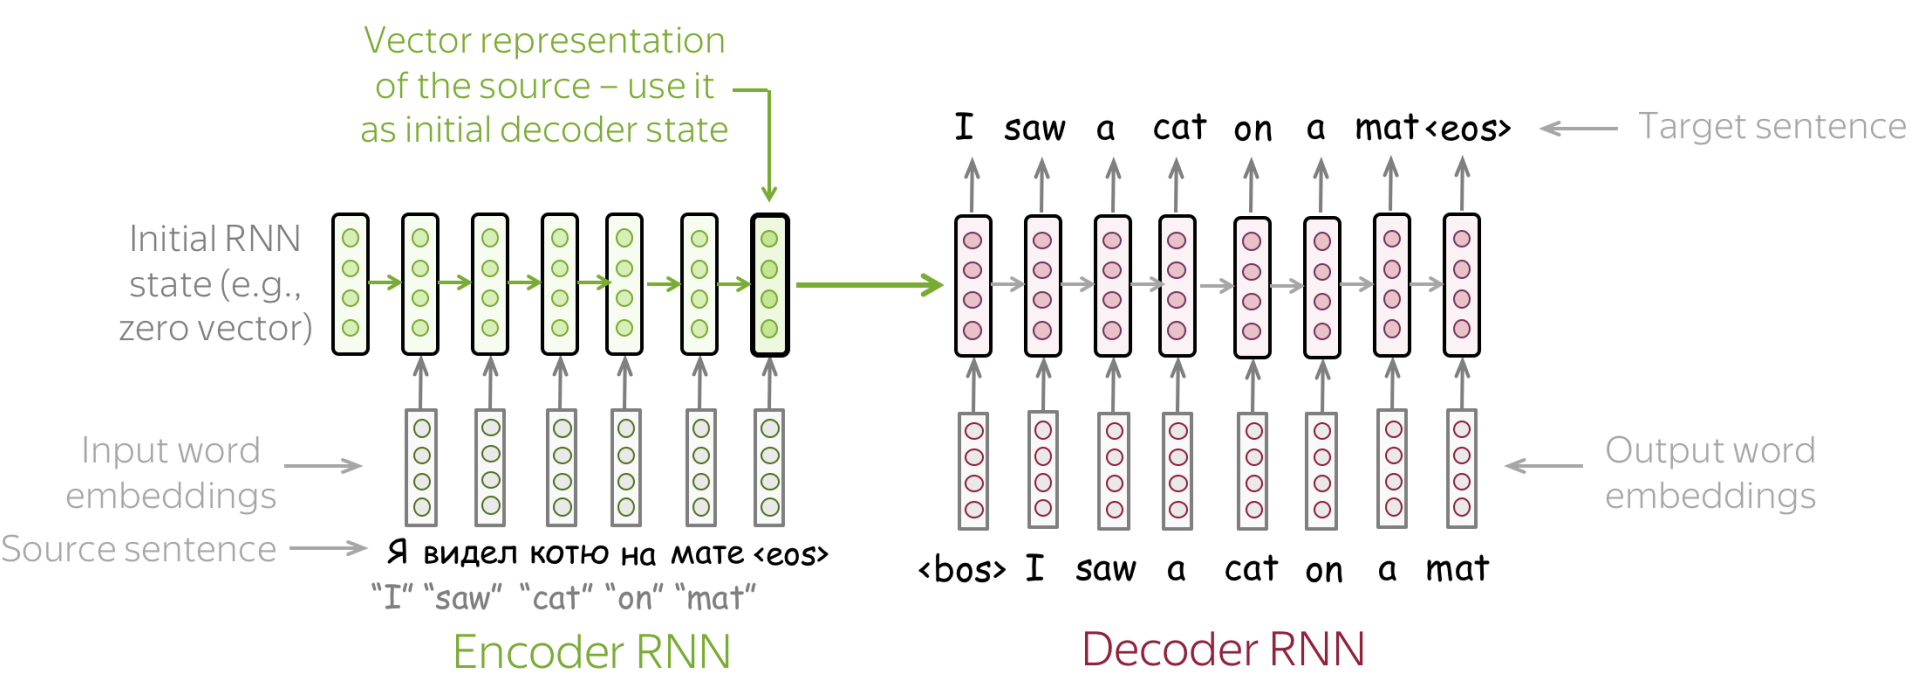
\includegraphics[width=0.3\textwidth]{media/seq2seqrnn.png}
\end{center}

\underline{Training}\\
Using cross entropy loss with the one-hot vector of the corect word as $p$. This gives a loss function
$$\operatorname{Loss}\left(p^*, p\right)=-\log \left(p_{y_t}\right)=-\log \left(p\left(y_t \mid y_{<t}, x\right)\right)$$
$x=\left(x_1, \ldots, x_m\right)$ := training input (source) sequence\\
$y=\left(y_1, \ldots, y_n\right)$ := training target (output) sequence\\

\underline{Greedy Decoding}: At each step, pick the most probable token.\\
This is a good baseline but inherintly flawed, the best token at the current step does not necessarily lead to the best sequence.\\

\underline{Beam Search}: At each step, keep track of the $k$ most probable sequences.\\
Usually, the beam size is 4-10. Increasing beam size is computationally inefficient and leads to worse quality.
\begin{center}
    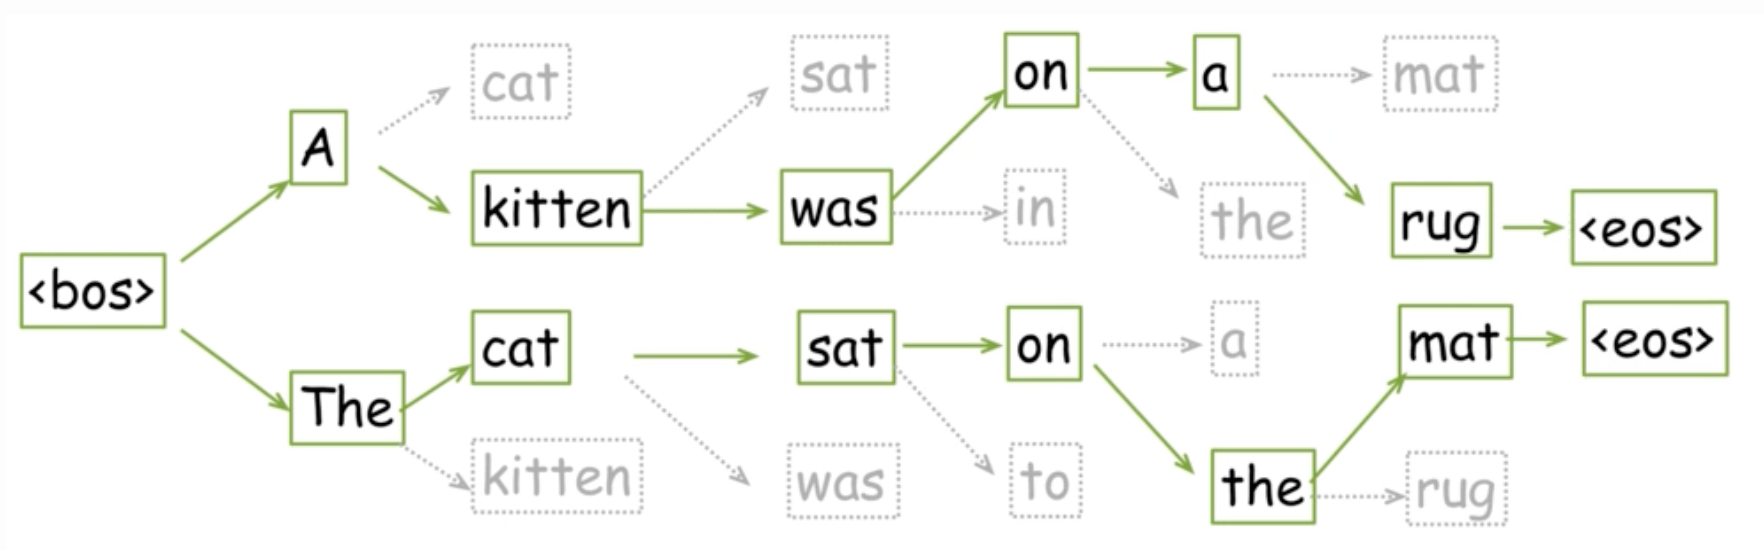
\includegraphics[width=0.3\textwidth]{media/beam-search.png}
\end{center}    

\subsubsection*{Encoder-Decoder Bottleneck}
\begin{itemize}[label=\textbullet, labelsep=0.3em, leftmargin=0.5em, itemsep=0em]
    \item for the encoder, it is hard to compress the sentence. It is likely to "forget" something. 
    \item for the decoder, different information may be relevant at different steps. The decoder sees only one representation of source.
\end{itemize}

\subsubsection*{Attention}
At different steps, let a model "focus" on different parts of the input.

The encoder does not have to compress the whole source into a single vector - it gives representations for all source tokens (for example, all RNN states instead of the last one).

For each decoder step
\begin{itemize}[label=\textbullet, labelsep=0.3em, leftmargin=0.5em, itemsep=0em]
\item receives attention input: a decoder state $h_t$ and all encoder states $s_1, s_2, \ldots, s_m$;
\item computes attention scores: given one decoder state and one encoder state, returns a scalar value representing the "relevence" of the encoder state
 $h_t$. $\operatorname{score}\left(h_t, s_k\right), \mathrm{k}=1 . . \mathrm{m}$ it  $\operatorname{score}\left(h_t, s_k\right)$
\item computes attention weights: apply \textbf{SoftMax} to attention scores
\item computes attention output: weighted vector sum of encoder states with attention weights.
\end{itemize}
\begin{center}
    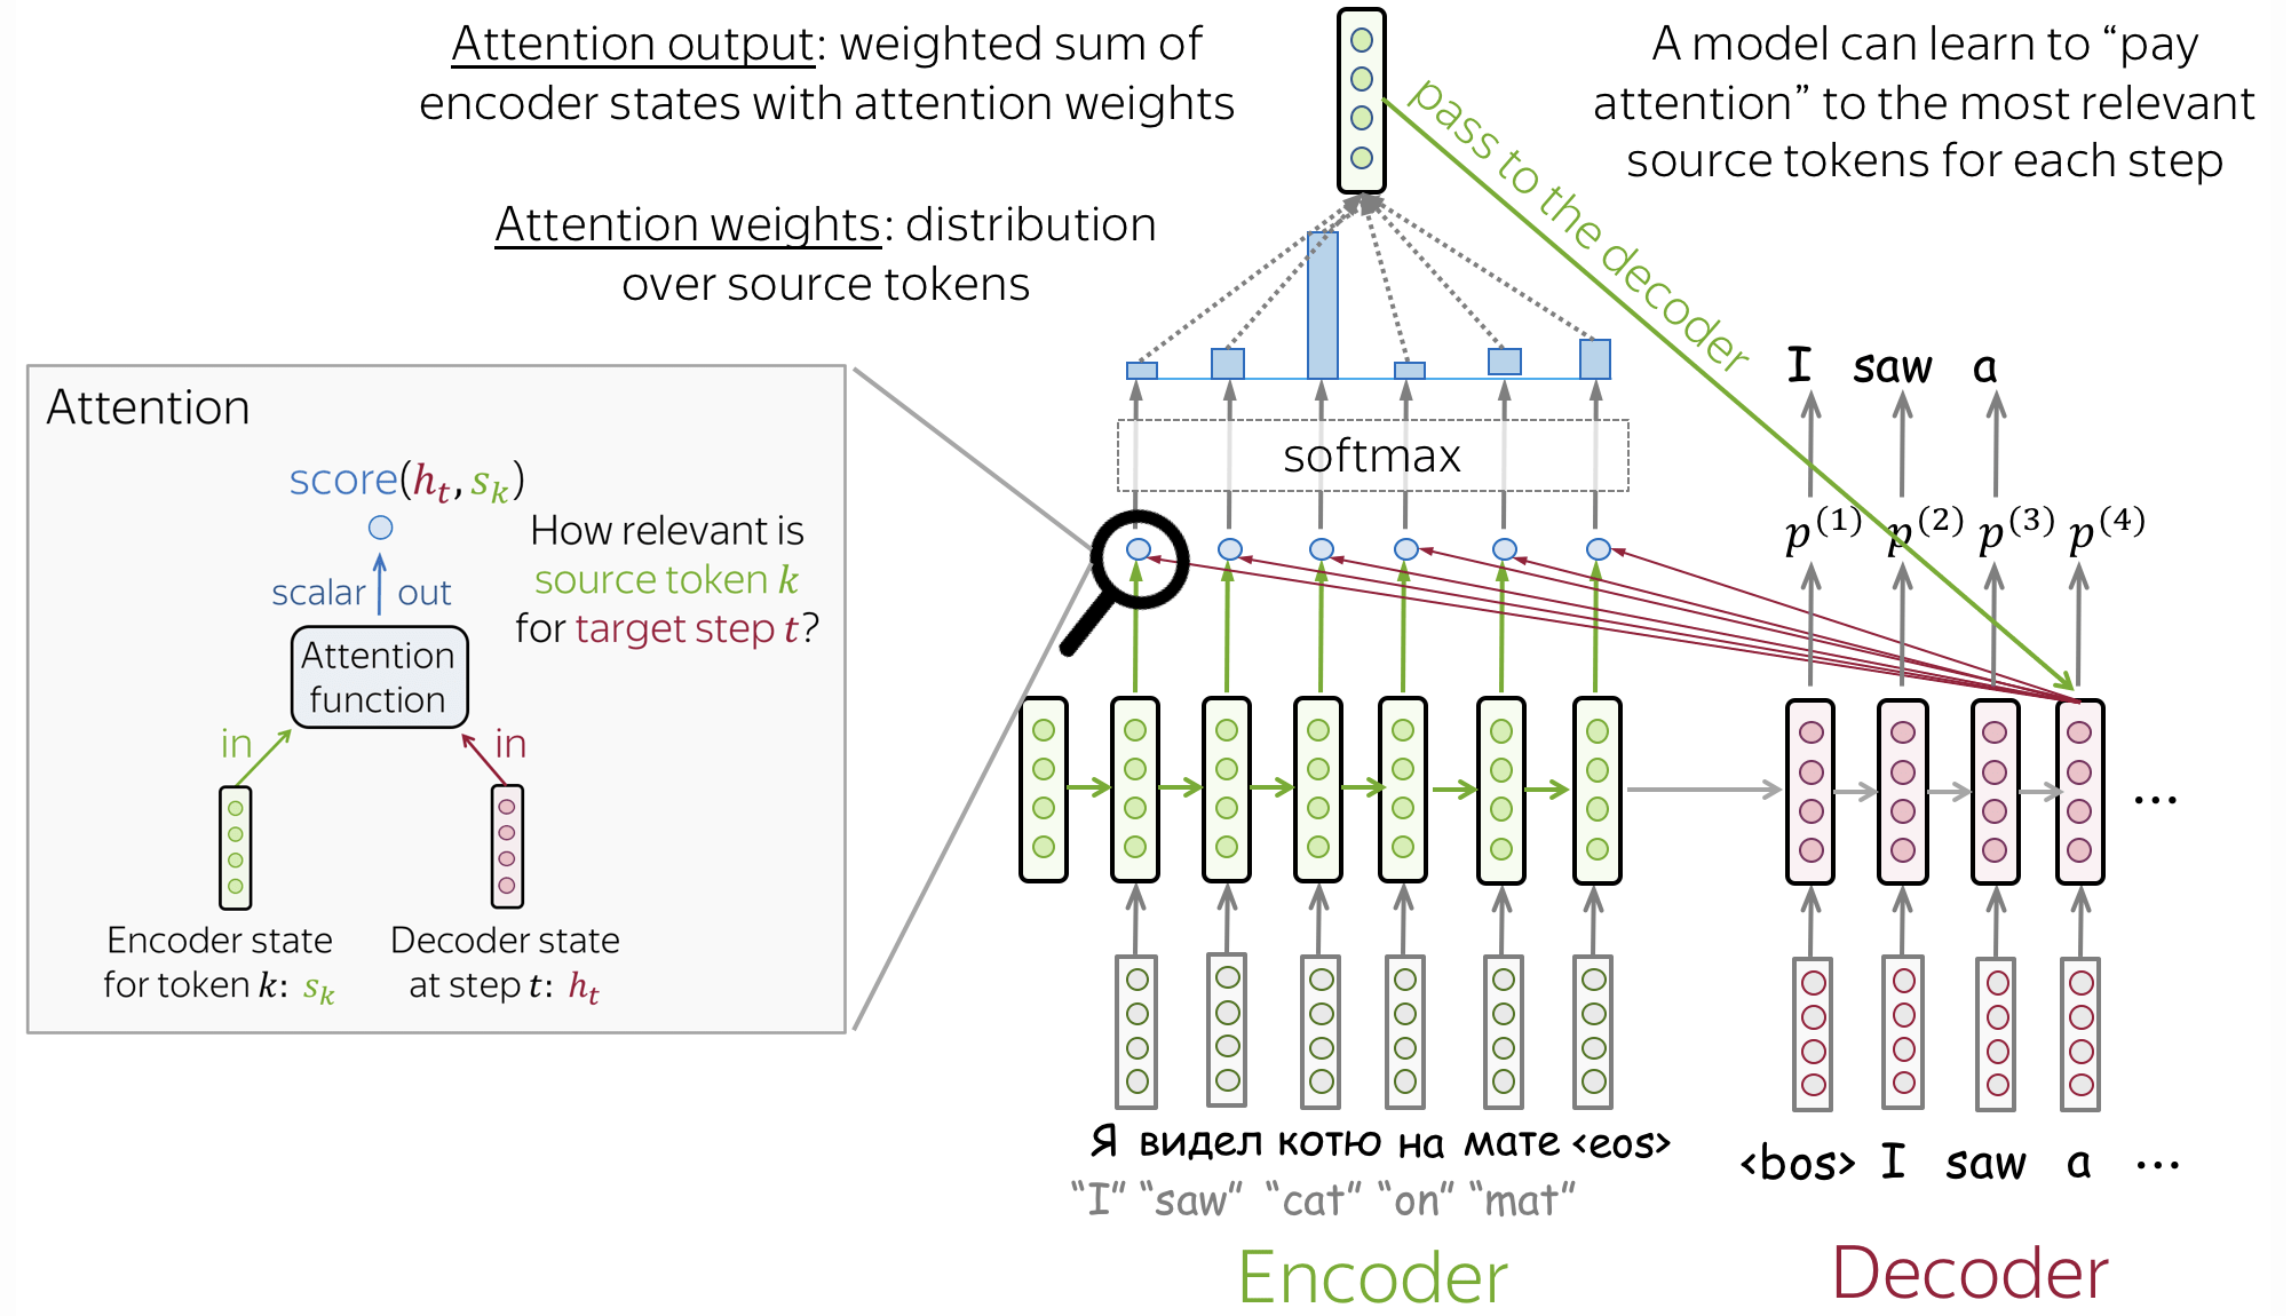
\includegraphics[width=0.32\textwidth]{media/attention.png}
\end{center}
\underline{Computing Attention}
\begin{center}
    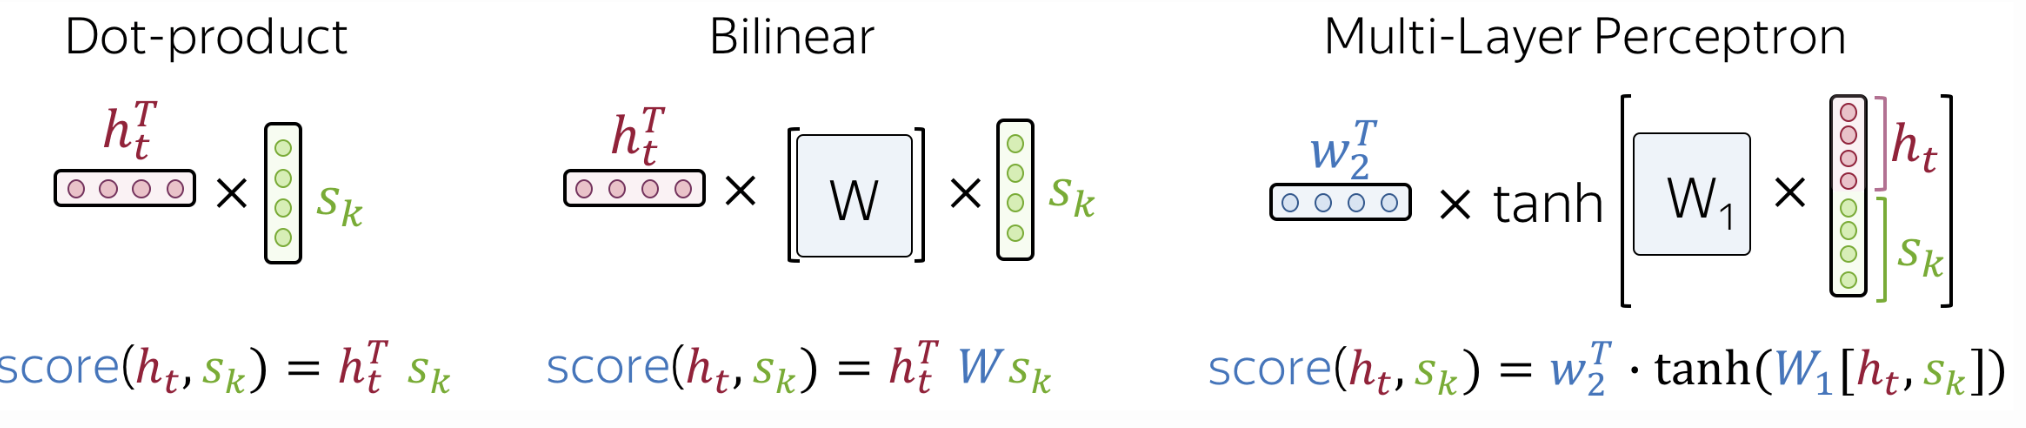
\includegraphics[width=0.32\textwidth]{media/comp-attention.png}
\end{center}

\subsubsection*{Transformers}
When encoding a sentence, RNNs won't understand it means until they read the whole sentence, and this can take a while for long sequences. 

In contrast, in Transformers' encoder tokens interact with each other all at once. Exchanging information to try and understand each other. \\

\underline{Self-Attention (Encoder)}\\
Self-attention is that self-attention operates between representations of the same nature: e.g., all encoder states in some layer.
\begin{center}
    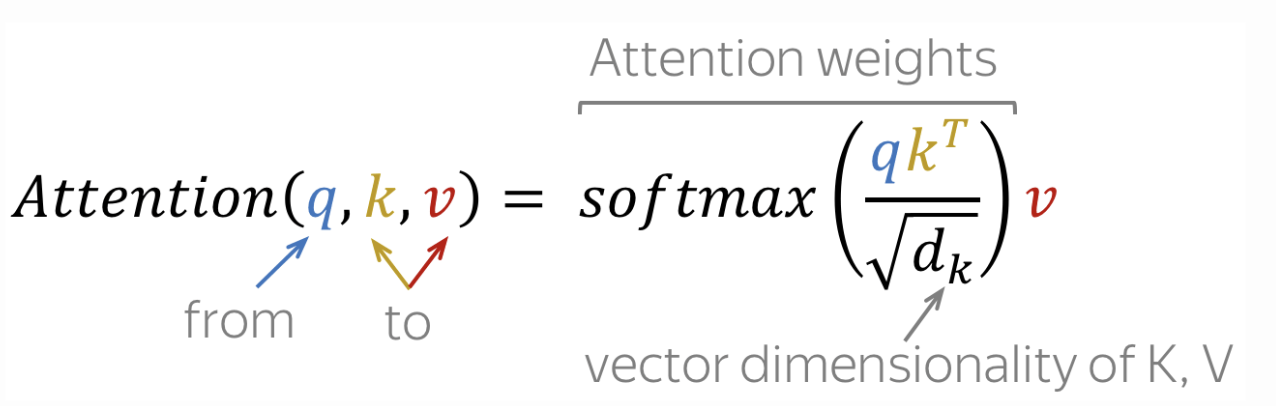
\includegraphics[width=0.35\textwidth]{media/attention-eq.png}
\end{center}

\underline{Query, Key, and Value}\\
Each encoder vector recieves three representations:
\begin{center}
    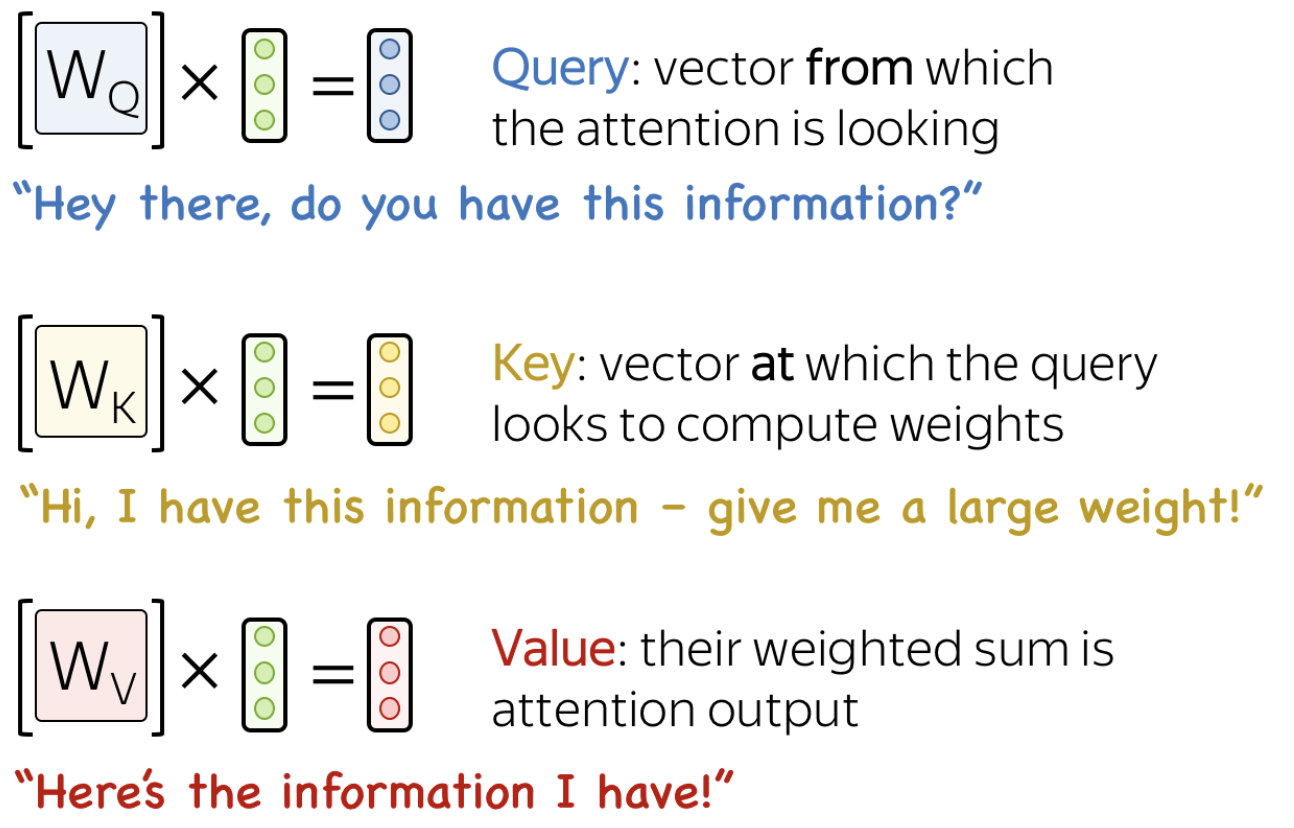
\includegraphics[width=0.35\textwidth]{media/key-query-value.png}
\end{center}

\underline{Masked Self-Attention (Decoder)}\\
Masking is the process of zeroing future vectors when conducting self-attention on the decoder vectors.\\

\underline{Multi-Head Attention}\\
Each word is part of varipus relations to other words.

Multi-Head Attention allows a model to focus on multiple things \textbf{simultaneously}. 

We use several heads and concatenate their outputs.

\underline{A Complete Transformer}
\begin{center}
    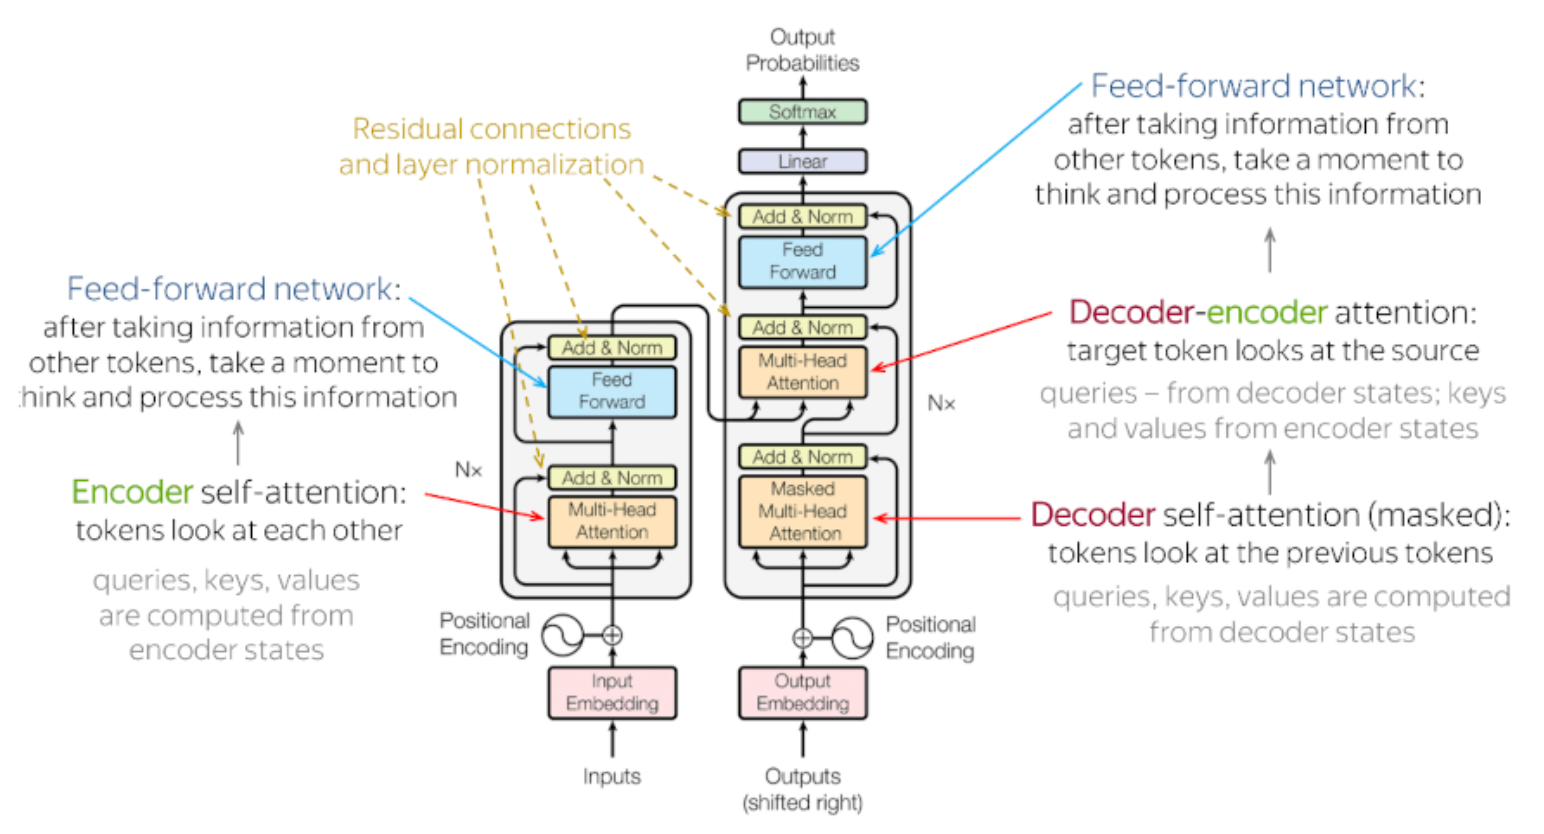
\includegraphics[width=0.35\textwidth]{media/transformer.png}
\end{center}

\textbf{Positional Encoding}\\
When using absolute value positional encodings, there will be many training examples for the low order encodings and fewer as we go higher. This can lead to the higher encodings being poorly trained, and may result in poor generalization.
\subsection*{Transfer Learning}
Typically we don't have enough data to estimate an accurate model.

Transfer learning lets us sue models trained on other datasets. 

The training data for specific tasks is often labelled, small and undiverse. \\
The training data for word embeddings is any text and so is more diverse massive. 
We can get a much more general knowledge base, which knows the relationships between words 
rather than being specifically trained to perform some task.

Can struggle with domain specific tasks so we can fine tune with task specific knowledge.

Rather than using these learned embeddings as the input for a task specific model, models like GPT and BERT are themselves so general that no task specificity is needed.

\end{multicols*}
\end{document}